%%%%%%%% ICLR 2027 CONFERENCE SUBMISSION FILE %%%%%%%%%%%%%%%%%
% Anonymous submission: \iclrfinalcopy must stay commented out.
% Ported 2026-09-16 from the TMLR-format source (paper/overleaf_update_20260916/).

\documentclass{article}

% Recommended, but optional, packages for figures and better typesetting:
\usepackage{microtype}
\usepackage{graphicx}
\usepackage{booktabs} % for professional tables
\usepackage{enumitem}


\newcommand{\N}{\mathbb{N}}
\newcommand{\MSE}{\mathsf{MSE}}
\newcommand{\R}{\mathbb{R}}
\newcommand{\Sys}{\mathfrak{S}}
\newcommand{\Xx}{\mathcal{X}}
\newcommand{\Yy}{\mathcal{Y}}
\newcommand{\seq}[1]{\langle #1 \rangle}
\newcommand{\Relu}{\mathsf{ReLU}}




\usepackage[T1]{fontenc}
\usepackage{iclr2027_conference,times}
\usepackage{url}
% hyperref makes hyperlinks in the resulting PDF.
\usepackage{hyperref}

% For theorems and such
\usepackage{amsmath}
\usepackage{amssymb}
\usepackage{mathtools}
\usepackage{amsthm}

% if you use cleveref..
\usepackage[capitalize,noabbrev]{cleveref}

% For highlighting additions in blue
\usepackage{xcolor}

%%%%%%%%%%%%%%%%%%%%%%%%%%%%%%%%
% THEOREMS
%%%%%%%%%%%%%%%%%%%%%%%%%%%%%%%%
\theoremstyle{plain}
\newtheorem{theorem}{Theorem}[section]
\newtheorem{proposition}[theorem]{Proposition}
\newtheorem{lemma}[theorem]{Lemma}
\newtheorem{corollary}[theorem]{Corollary}
\theoremstyle{definition}
\newtheorem{definition}[theorem]{Definition}
\newtheorem{assumption}[theorem]{Assumption}
\theoremstyle{remark}
\newtheorem{remark}[theorem]{Remark}
\theoremstyle{plain}
\newtheorem*{lemmastar}{Lemma}
\newtheorem*{assumptionstar}{Assumption}

% Todonotes is useful during development; simply uncomment the next line
%    and comment out the line below the next line to turn off comments
\setlength{\marginparwidth}{2cm}
\usepackage[disable,textsize=tiny]{todonotes}


\title{Monotonicity as an Architectural Bias for Robust Language Models}

\author{Anonymous authors \\ Paper under double-blind review}

%\iclrfinalcopy % Uncomment ONLY for the camera-ready version, after acceptance.

\setlength{\textfloatsep}{8pt plus 2pt minus 2pt}
\setlength{\abovecaptionskip}{4pt}
\setlength{\belowcaptionskip}{2pt}

\begin{document}

\maketitle

\begin{abstract}

Large language models (LLMs) remain strikingly brittle under adversarial
prompts and jailbreak attacks: small, carefully chosen perturbations can
produce large and unpredictable changes in internal representations and
generated outputs. We introduce \emph{monotonicity} as an architectural
inductive bias for improving the robustness of Transformer language models.
Rather than constraining the entire network, we impose monotonicity selectively
within feed-forward sublayers, where semantic representations are nonlinearly
refined, while leaving attention unconstrained to preserve contextual
reasoning, negation, and contradiction. This separation yields
\emph{monotone language models} whose semantic refinement is order-preserving
without globally restricting Transformer expressivity.
On an encoder--decoder model (T5), this simple structural constraint substantially
improves adversarial robustness while largely preserving task performance:
gradient-based attack success rates fall from $60\%$ for an identically
fine-tuned unconstrained baseline ($69\%$ for the pretrained model) to $17\%$,
with a modest reduction in summarization quality (a $2$--$5\%$ relative ROUGE-L
decrease on two benchmarks, consistent across five training seeds on full test sets), without adversarial
training, additional data, or modified training objectives. We further show that
the effect transfers to the decoder-only Pythia-1.4B architecture, but only when
the constraint is placed along the relevant propagation paths. Constraining the
feed-forward input projection alone is ineffective, whereas constraining both
projections reduces mean attack success from $69.0\%$ to $42.5\%$ across three
seeds, at a markedly larger cost in clean perplexity; the advantage persists
under random-substitution and gradient-free query attacks, arguing against
gradient masking as the explanation. Together, these results identify
monotonicity as a practical structural prior for robust language modeling and
show that its effectiveness depends critically on where constraints are imposed
within the architecture. %, revealing an architecture-dependent trade-off between robustness and model quality.

% Our results demonstrate that strong architectural constraints, long assumed to limit the capacity of LLMs, can be applied at scale without sacrificing accuracy. Monotonicity thus emerges as a practical and principled design choice for building language models whose semantic behavior is more robust, predictable, and amenable to formal reasoning.
\end{abstract}

\section{Introduction}
\label{sec:intro}

Large language models (LLMs) achieve remarkable performance across language tasks, yet their behavior remains surprisingly brittle: carefully crafted prompts, jailbreaks, and even small targeted perturbations can push otherwise well-aligned models toward unsafe or unintended outputs. This vulnerability is not merely a failure of alignment; it reflects a deeper property of neural language models, whose representations evolve in extremely high-dimensional spaces where small input changes can be amplified through successive layers, a sensitivity linked in part to the large Lipschitz constants of Transformers~\citep{newhouse2025training}. Existing approaches to robustness~\citep{wei2023jailbroken, su2024mission} largely rely on training-time interventions such as alignment objectives~\citep{cao2024defending} and adversarial training~\citep{howe2024effects}, or on inference-time defenses such as output filtering~\citep{khachaturov2025adversarial}; while effective in many settings, they are typically reactive, suppressing undesirable behavior after the underlying vulnerability has emerged. This raises a fundamental question: \emph{can robustness be built into the architecture itself, rather than added only after vulnerabilities are discovered?}

We explore \emph{monotonicity} as such a structural inductive bias. Monotonicity imposes directional consistency: strengthening an input along an ordered dimension cannot cause the corresponding downstream representation to move in the opposite direction. This property has a long history in machine learning~\citep{Gupta2016MonotonicLattices, runje2023constrained} and in control theory, where monotone systems admit tractable reasoning about stability and perturbation propagation in high-dimensional settings~\citep{smith1995monotone,michel2015stability,ito2014max,rantzer2014control}. It has a natural interpretation in language models: adding supporting evidence should not weaken a conclusion, adding safety constraints should not produce a less constrained internal state, and increasing the stated severity of a situation should not make the model more permissive. A sequence of prompts that progressively strengthens a claim,
\emph{``The medication has side effects''}
$\preceq$
\emph{``The medication has severe side effects''}
$\preceq$
\emph{``The medication has severe side effects and requires medical supervision''},
induces a natural partial order over meaning, and ideally the model's internal representations should preserve this ordering rather than allow stronger information to produce weaker or contradictory downstream states. Contemporary language models often violate this expectation, and we argue that the instability lies in how semantic information is transformed inside the network, not only in the input space.

This perspective suggests a structural source of brittleness. Transformers alternate between contextual aggregation through attention, which is naturally suited to explicit contextual operations such as negation, contrast, and exception, and nonlinear feed-forward transformations, which are largely unconstrained and can amplify, suppress, or reverse semantic features in ways that are difficult to predict; we hypothesize that these unconstrained reversals create exploitable directions through which small adversarial perturbations can be amplified. Our motivation mirrors \emph{monotone Boolean circuits}~\citep{jukna2012boolean}, in which negation is excluded from the internal computation and must be introduced explicitly at the input: by enforcing monotonicity only during semantic refinement, we encourage negation, contradiction, and constraint relaxation to arise through attention rather than through fragile cancellation inside nonlinear transformations. The resulting Transformer is not globally monotone, nor does the constraint eliminate all adversarial behavior; it imposes structure precisely where semantic features are refined.

Our central finding is that monotonicity can be incorporated into Transformer architectures at a modest cost in task performance in the encoder--decoder setting, and at a markedly larger cost in clean perplexity in the decoder-only setting, while the resulting models achieve substantially greater robustness in both settings, without adversarial training, additional data, modified training objectives, or heuristic defenses (whether the robustness gain stems from the constraint or from its initialization remains open; Appendix~\ref{app:ablation} settles this only for clean quality). Selectively imposed monotonicity is thus a practical inductive bias at an architecture-dependent rather than prohibitive cost, contrary to the assumption that strong structural restrictions must sacrifice optimization or expressive power~\citep[see][]{sartor2025advancing}.

\noindent\textbf{Contributions.}
\vspace{-0.5em}
\begin{enumerate}[leftmargin=*,itemsep=0pt,topsep=2pt]
    \item \textbf{Selective monotonicity for Transformers.} Monotone feed-forward sublayers that enforce order-preserving semantic refinement while leaving attention unconstrained.
    \item \textbf{Practical monotone language models.} Pretrained Transformers can be converted into monotone counterparts that retain competitive downstream performance in the encoder--decoder setting.
    \item \textbf{Substantial gains in adversarial robustness.} Monotonicity significantly reduces vulnerability to gradient-based token-level attacks (HotFlip; more weakly, universal triggers); on the decoder-only track the reduction persists under random-substitution and gradient-free query attacks, arguing against gradient masking.
    \item \textbf{Architecture-dependent constraint placement.} On Pythia-1.4B the benefit transfers under the same constraint scope (both feed-forward projections), constraining the input projection alone is ineffective, and the clean-performance cost is markedly larger.
\end{enumerate}

\section{Related Work}
\label{sec:related}
\textbf{Vulnerabilities and defenses.}
LLMs are highly susceptible to manipulations that bypass alignment, including transferable adversarial suffixes~\citep{Zou2023UniversalTransferableAttacksOnAlignedLLMs}, position-sensitive~\citep{wang2025vulnerability}, interpretable~\citep{Zhu2023AutoDAN}, many-shot~\citep{anil2024many}, and multilingual~\citep{deng2024multilingual} jailbreaks, and prompt injection~\citep{li2025security}; they also perform poorly under systematic adversarial evaluation~\citep{Wang2021AdvGLUE}. The token-level attacks we use descend from gradient-guided substitutions~\citep{ebrahimi2018hotflip}, universal triggers~\citep{wallace2019universal} and their descendants~\citep{shin2020autoprompt,guo2021gradient}, gradient-free query-based substitutions~\citep{jin2020bert}, and attacks on sequence-to-sequence models~\citep{cheng2020seq2sick}. Defenses include smoothing with provable guarantees~\citep{Robey2023SmoothLLM}, prompt classifiers~\citep{sayeedi2025jailbreaktracer}, adversarial training~\citep{howe2024effects}, perplexity filtering~\citep{jain2023baseline}, representation-level interventions~\citep{zou2024circuit}, and certified training~\citep{jia2019certified}; most remain reactive and training-dependent. Since apparent robustness to gradient-based attacks can be an artifact of obfuscated gradients~\citep{athalye2018obfuscated,carlini2019evaluating,tramer2020adaptive}, our controls include gradient-free attacks (Section~\ref{sec:results-pythia}).

\textbf{Monotonic networks and structural constraints.}
Nonnegative-weight sigmoidal networks~\citep{Daniels2010Monotone} and min--max networks of constrained linear units~\citep{Sill1998MonotonicNetworks} are universal approximators of monotone functions; practical monotone architectures include lattice models~\citep{Gupta2016MonotonicLattices,You2017DeepLattice}, certified or counterexample-guided constructions~\citep{liu2020certified,sivaraman2020counterexample}, integrated positive-derivative networks~\citep{wehenkel2019unconstrained}, smooth min--max networks~\citep{igel2024smooth}, and Lipschitz-bounded residual architectures that certify robustness~\citep{nolte2023expressive,kitouni2023robust}; the depth and width price of nonnegative parameters is known~\citep{mikulincer2022size}. Monotone classifiers were shown to resist a class of evasion attacks before the LLM era~\citep{incer2018adversarially}; monotone dynamical systems have order-preserving flows with strong convergence properties~\citep{hirsch2006monotone,angeli2003monotone}; structured layers~\citep{Amos2017OptNet} and Lipschitz control of attention~\citep{kim2021lipschitz,newhouse2025training} are related routes to robustness (see Appendix~\ref{app:related}).

\section{Monotone Transformers}
\label{Prelim}
We study monotonicity constraints in a Transformer sequence-to-sequence model $\mathcal{M}_\theta : \mathcal{X} \to \mathcal{Y}$ from input token sequences to output token sequences, composed of attention layers, feed-forward network (FFN) sublayers, residual connections, and normalization. We define the order along which monotonicity is required, then the constrained sublayer, then how the constraint is enforced; proofs and details are in Appendices~\ref{app:proofs} and~\ref{app:model-details}.

\textbf{Semantic order.}
Fix $A \in \mathbb{R}^{p \times d}$ whose rows define interpretable semantic axes.
For a hidden state $h \in \mathbb{R}^d$, define semantic coordinates $s := Ah \in \mathbb{R}^p$
and equip $\mathbb{R}^p$ with the standard product order. We define a preorder on
$\mathbb{R}^d$ by $h \preceq h' \Longleftrightarrow Ah \le Ah'$ (elementwise)
and interpret $h' \succeq h$ as semantically stronger along the chosen axes (when $A = I$, $\preceq$ is the coordinatewise order).
In practice, $A$ may be chosen by training $p$ linear probes on ordered prompt pairs or from fixed directions of auxiliary classifiers, and is fixed before imposing constraints. \emph{All models trained in this paper use $A = I$}, so that $g$ below is the model's own FFN and every FFN weight is constrained; probe-derived directions serve only as a post-hoc diagnostic (Section~\ref{sec:results-order}). The general construction makes the role of $A$ explicit: with $p < d$ it selects a semantic subspace along which monotonicity holds, leaving $\ker(A)$ unconstrained, and $A$-monotonicity of the sublayer follows from that of the constrained multilayer perceptron (MLP) $g$ alone (Proposition~\ref{prop:amono}).

\begin{definition}[Monotonicity]
\label{def:monotone}
A function $f : \mathbb{R}^n \to \mathbb{R}^m$ is \emph{monotone} (or \emph{coordinatewise monotone}) if $x \le x'$ implies $f(x) \le f(x')$ for all $x, x' \in \mathbb{R}^n$; equivalently, $f$ is non-decreasing in each input coordinate with the others held fixed. A function $F:\mathbb{R}^d \to \mathbb{R}^d$ is \emph{$A$-monotone} if $h \preceq h' \Rightarrow F(h) \preceq F(h')$, i.e., $Ah \le Ah' \Rightarrow AF(h) \le AF(h')$.
\end{definition}

\begin{lemma}[Closure under Composition]
\label{lem:mono_comp}
If $f : \mathbb{R}^n \to \mathbb{R}^m$ and $g : \mathbb{R}^m \to \mathbb{R}^k$ are monotone, then $g \circ f$ is monotone.
\end{lemma}

\textbf{Semantic-monotone FFN sublayer.}
Assume $A$ has full row rank and let $A^\dagger \in \mathbb{R}^{d \times p}$ be a fixed right inverse of $A$ (e.g., $A^\dagger = A^\top(AA^\top)^{-1}$), so that $A A^\dagger = I_p$, and define the FFN update
\[
F(h) := h + A^\dagger\, g(Ah), \qquad g:\mathbb{R}^p \to \mathbb{R}^p \text{ coordinatewise monotone.}
\]

\begin{proposition}[Sufficient condition for $A$-monotonicity]
\label{prop:amono}
If $g$ is monotone w.r.t.\ the product order on $\mathbb{R}^p$, then $F$ is $A$-monotone.
In particular, it suffices that $g$ is an MLP with elementwise non-decreasing activations
and elementwise nonnegative weight matrices.
\end{proposition}

\begin{proposition}[Sufficient Condition for FFN Monotonicity]
\label{prop:ffn_mono}
Let $N : \mathbb{R}^{n_0} \to \mathbb{R}^{n_{k+1}}$ be a feed-forward network $y_0 = u$, $y_{i+1} = \sigma(W_i y_i + b_i)$ ($i = 0,\ldots,k-1$), $N(u) = W_k y_k + b_k$, with $W_i \in \mathbb{R}^{n_{i+1}\times n_i}$ and $\sigma$ applied elementwise. If $\sigma$ is non-decreasing and $W_i \ge 0$ for $i = 0,\ldots,k$, then $N$ is monotone.
\end{proposition}
\textit{Proof.} Each affine map $y \mapsto W_i y + b_i$ with $W_i \ge 0$ is monotone, as is the elementwise map $y \mapsto \sigma(y)$ because $\sigma$ is non-decreasing; the claim follows by Lemma~\ref{lem:mono_comp}. \hfill $\square$

Such \emph{monotone neural networks} are universal approximators of continuous monotone functions on compact domains when the activation is bounded and sigmoidal~\citep{Daniels2010Monotone}; this does not extend to ReLU, for which every output coordinate of a nonnegative-weight network is convex in its input~\citep{runje2023constrained}, so the ReLU-based monotone FFNs of our T5 experiments are a strictly restricted family; whether this restriction, rather than the initialization, costs clean quality is examined in Appendix~\ref{app:ablation}.

\begin{definition}[Monotone Transformer]
\label{def:mono_transformer}
A Transformer $\mathcal{M}_\theta$ is \emph{$A$-monotone with respect to its feed-forward sublayers}
if each FFN sublayer implements an update $F(h) := h + A^\dagger\, g(Ah)$ with $A^\dagger$ a fixed right inverse of $A$ and $g:\mathbb{R}^p\to\mathbb{R}^p$ coordinatewise monotone (e.g., an MLP with elementwise non-decreasing activations and elementwise nonnegative weight matrices). All other components (attention, residuals, normalization) are left unconstrained.
\end{definition}

This definition does not assert global monotonicity of the full Transformer; it enforces monotonic refinement at the level of FFN sublayers, where we hypothesize that implicit feature cancellation is most likely to occur (cf.~\citealp{runje2023constrained,sartor2025advancing,nguyen2023mononet}). In the pre-normalized T5 and GPT-NeoX blocks we instantiate, the branch receives $u = \mathrm{LN}(h)$ (layer normalization) and the residual is added outside it, $F(h) = h + g(\mathrm{LN}(h))$, so $F$ itself need not be monotone in $h$; the property we enforce, and analyze in Section~\ref{sec:gradient-attenuation}, is the monotonicity of the branch $g$ as a map of its own input $u$ (Remark~\ref{rem:preln}).

\textbf{Enforcing the constraint.}
We constrain all linear maps inside $g$ to be elementwise nonnegative and keep the model's own activation: the non-decreasing ReLU in the T5 track, and in the Pythia track GELU, which is non-decreasing only outside a small region (Section~\ref{sec:setup-pythia}). Each constrained weight matrix is reparameterized as $W = \phi(V)$ with $\phi(v) = \log(1+\exp(v))$ applied elementwise to an unconstrained $V$, which maintains $W \ge 0$ throughout optimization without projection. To retain the pretrained weights we initialize $V_{\mathrm{init}} = \phi^{-1}(|W_{\mathrm{pre}}| + \epsilon)$, $\epsilon = 10^{-4}$, which preserves the magnitude of every pretrained weight while flipping the sign of the negative entries; recovering from this sign disruption is the task of the subsequent fine-tuning, and its cost is isolated in Appendix~\ref{app:ablation}. Pretrained biases are retained unconstrained.

\section{Experimental Setup}
\label{sec:setup}
Full protocols (hyperparameters, datasets, decoding, attack budgets, controls, and the order-preservation corpus) are in Appendices~\ref{app:training}, \ref{app:pythia}, and~\ref{app:protocols}.

\textbf{Encoder--decoder track (T5).}
We instantiate Definition~\ref{def:mono_transformer} with $A = I_d$ on \texttt{T5-small}~\citep{raffel2020exploring} (6 encoder and 6 decoder layers, $d = 512$, 8 heads, 2048-dimensional FFNs): each FFN sublayer keeps its pretrained architecture, $g(u) = W_{\mathrm{o}}\,\mathrm{ReLU}(W_{\mathrm{i}} u)$ with $W_{\mathrm{i}}\in\mathbb{R}^{2048\times 512}$ and $W_{\mathrm{o}}\in\mathbb{R}^{512\times 2048}$ both constrained through the softplus reparameterization in all 12 blocks (25M of 60.5M parameters, 42\%), so that $g$ is a monotone network in the sense of Proposition~\ref{prop:ffn_mono}. The \emph{baseline} is the same checkpoint fine-tuned identically without the constraint; the \emph{standard} model is the pretrained checkpoint. Fine-tuning uses other summarization corpora (Appendix~\ref{app:training}); all three models are evaluated out of distribution on the full CNN/DailyMail and XSUM test sets over five training seeds.

\textbf{Attacks (T5).}
\label{sec:setup-attacks}
\emph{Universal adversarial triggers} (UATs)~\citep{wallace2019universal} are short, input-agnostic token sequences that, when prepended to an input, maximize the model's loss; we optimize five-token triggers by coordinate-wise search (five restarts, 100 iterations) on 1{,}000 held-out validation examples and evaluate them on 1{,}500 disjoint test examples. Because the trigger is prepended and the encoder input is then left-truncated to 512 tokens, the trigger is discarded for articles longer than about 505 tokens, so the T5 trigger results are a lower bound (Appendix~\ref{app:protocols}). \emph{HotFlip}~\citep{ebrahimi2018hotflip} replaces up to five tokens per example, chosen from the gradient of the loss with respect to token embeddings, with the vocabulary items that maximize the first-order loss increase. Robustness is quantified by the relative increase in cross-entropy loss under attack (\emph{degradation}, averaged over examples), the attack success rate (degradation above 10\%), and independent-samples $t$-tests on per-example degradations; since relative degradation is normalized by each model's own clean loss, we also report the absolute increase in nats. For UATs we report the relative negative log-likelihood (NLL) increase.

\textbf{Order-preservation diagnostic.}
To test whether sublayer monotonicity yields order preservation along the semantic directions that motivate it, we build a templated corpus of ordered prompt pairs (13 semantic axes on 18 topics; 702 adjacent-level pairs from four-level chains, split by chain into 507 probe-fitting and 195 evaluation pairs), fit $p = 64$ bootstrap logistic-regression probe directions $A$ per model on final-layer representations (mean- or last-token-pooled) of the fitting split, and report at every layer the fraction of probe coordinates with $A h_{\mathrm{weak}} \le A h_{\mathrm{strong}}$ on evaluation pairs; the probe is fit post hoc and plays no role in training.

\textbf{Decoder-only track (Pythia-1.4B).}
\label{sec:setup-pythia}
To test generalization to decoder-only architectures, we repeat the study on Pythia-1.4B~\citep{biderman2023pythia}, a 24-layer GPT-NeoX model with $d = 2048$, fine-tuned and evaluated on the (uncopyrighted) Pile~\citep{gao2020pile} with clean performance measured by held-out perplexity. Each block has an attention output projection and an MLP with projections $W_{\mathrm{in}} \in \mathbb{R}^{4d \times d}$ and $W_{\mathrm{out}} \in \mathbb{R}^{d \times 4d}$; since decoder-only blocks lack T5's encoder--decoder bottleneck, we compare three \emph{constraint scopes} applied in all 24 layers with $A = I$: \textbf{MLP-in} ($W_{\mathrm{in}}$ only), \textbf{MLP-both} ($W_{\mathrm{in}}$ and $W_{\mathrm{out}}$, the direct analogue of the T5 scheme), and \textbf{MLP-in + Attn-out} ($W_{\mathrm{in}}$ and the attention output projection). Two caveats apply: GELU is not globally non-decreasing ($\mathrm{GELU}'(z) < 0$ for $z < -0.752$, with minimum $\approx -0.13$), so the constrained Pythia FFNs are monotone only up to this small region and the track tests the same weight constraint rather than an exactly monotone model; and only MLP-both constrains every FFN matrix, so the other scopes are ablations.

After imposing constraints, each model and an unconstrained \emph{baseline} undergo \emph{recovery training} on the Pile, the monotone runs with a larger budget (learning rate $5\times 10^{-5}$ vs.\ $10^{-5}$, warmup 20\% vs.\ 10\%, 10 vs.\ 5 epochs) to compensate for its disrupted initialization; scopes are screened on one seed (MLP-in at full budget, the others at a reduced budget, so the comparison is indicative) and the selected scope is validated at full budget on three seeds.

\textbf{Attacks and controls (Pythia).}
Robustness is assessed with causal-LM analogues of the T5 attacks (HotFlip, $n = 200$, up to 10 flips, success threshold 15\%; ten-token UATs, three restarts, 50 iterations, optimized on 80 and evaluated on 120 texts), with attack effect measured as the relative increase in mean per-token NLL of the perturbed sequence; since the inserted or substituted tokens are themselves prediction targets, absolute figures in this track are inflated by their low likelihood, although comparisons between the two models remain valid.

To distinguish robustness from gradient masking we add three controls: \emph{substitution transfer} (substitutions found on one model replayed against the other; likewise for triggers), a \emph{random-substitution control} (the same number of substitutions at random positions, with no model or gradient involved), and a \emph{gradient-free query attack} (greedy search over 20 candidates at each of 10 random positions, scored by the target model's own loss).

\section{Mechanisms of Gradient Attenuation in Monotone Feed-Forward Networks}
\label{sec:gradient-attenuation}
We propose a candidate mechanism for the empirical robustness gains: rather than claiming global guarantees, we analyze how monotonicity alters the local gradient structure of feed-forward sublayers in a way that can reduce the effectiveness of gradient-based attacks such as HotFlip. The analysis is motivated by monotone dynamical systems, in which cooperative interactions restrict the directions along which trajectories evolve~\citep{hirsch1985systems}; a network is not such a system, but the analogy suggests that monotonicity can limit the active directions along which outputs and gradients vary (Appendix~\ref{app:mechanism-details}). Proofs are in Appendices~\ref{app:proofs} and~\ref{app:mechanism-details}.

Consider an $A$-monotone update $F(h) = h + A^\dagger g(Ah)$ with $s := Ah$ and the induced semantic refinement map $T(s) := AF(h) = s + g(s)$. In our experiments $A = I$ and the FFN branch acts on the normalized state $u = \mathrm{LN}(h)$ (Remark~\ref{rem:preln}), so we take $s := u$ as the branch input and $g$ as the branch itself; because the block is pre-normalized, the Jacobian of the sublayer map $h \mapsto h + g(\mathrm{LN}(h))$ is $I_d + J_g(\mathrm{LN}(h))\,J_{\mathrm{LN}}(h)$ rather than $J_T = I + J_g$, so the correction term below acquires the unconstrained factor $J_{\mathrm{LN}}(h)$; all statements below concern the branch factor $J_g$.

\begin{lemma}[Non-negativity of the Semantic Jacobian]
\label{lem:jacobian-nonneg}
Let $g$ be an MLP with elementwise non-decreasing activation $\sigma$ and elementwise nonnegative weight matrices. At every $s$ at which $g$ is differentiable (all $s$ for $\sigma \in C^1$; almost every $s$ for ReLU), $J_T(s) = I + J_g(s)$ has non-negative entries (the same holds for every element of the Clarke generalized Jacobian and for the matrix returned by automatic differentiation; Appendix~\ref{app:mechanism-details}).
\end{lemma}

For a two-layer $g(s)=W_2\sigma(W_1 s + b_1)+b_2$, $J_g(s)=W_2\,\mathrm{diag}(\sigma'(W_1 s+b_1))\,W_1 \ge 0$ elementwise (deeper $g$ gives a product of nonnegative matrices): increasing any semantic coordinate cannot decrease any output coordinate through $T$, so sign cancellations are ruled out \emph{within semantic space}. Writing $\ell$ for the loss as a function of the sublayer output and $\nabla_{s'}\mathcal{L} := (A^\dagger)^\top \nabla\ell$ for the downstream gradient in semantic coordinates, the chain rule gives $\nabla_h \ell(F(h)) = \nabla\ell + A^\top J_g^\top \nabla_{s'}\mathcal{L}$: the residual path is unaffected by the constraint, and the semantic-space gradient $\nabla_s\mathcal{L}(T(s)) := J_T^\top \nabla_{s'}\mathcal{L} = \nabla_{s'}\mathcal{L} + J_g^\top \nabla_{s'}\mathcal{L}$ adds a correction $J_g^\top \nabla_{s'}\mathcal{L}$ whose matrix is nonnegative (Lemma~\ref{lem:jacobian-nonneg}), which rules out sign cancellation inside the correction but does not by itself reduce its magnitude ($J_T \ge I$).

\textbf{Saturation-induced attenuation.}
A hidden unit whose activation is flat at its current pre-activation contributes nothing to the gradient flowing through it; the assumption below fixes what ``flat'' means for our activations, and the lemma quantifies the contribution of nearly flat units.

\begin{assumption}[Saturating Activations]
\label{ass:saturation}
The activation $\sigma$ inside $g$ has bounded derivative and saturates in the negative direction: $|\sigma'(z)| \to 0$ as $z\to -\infty$, with $|\sigma'|$ non-decreasing on a tail $(-\infty, z^\ast]$. This holds for ReLU ($\sigma'(z) = 0$ for $z < 0$, $z^\ast = 0$), softplus and the logistic function ($z^\ast \le 0$), and GELU ($z^\ast = -\sqrt{2}$); ReLU, softplus, and GELU do not saturate in the positive direction ($\sigma' \to 1$), and only negative-tail saturation is used below.
\end{assumption}

\begin{lemma}[Gradient Attenuation under Saturation]
\label{lem:gradient-attenuation}
Let $T(s)=s+g(s)$ with $g(s)=W_2\sigma(W_1 s+b_1)+b_2$, $W_1\in\mathbb{R}^{m\times p}$ and $W_2\in\mathbb{R}^{p\times m}$ elementwise nonnegative, and $z_j(s) := (W_1 s + b_1)_j$. Wherever $\sigma$ is differentiable at $z(s)$, $J_g(s) = \sum_{j=1}^{m} \sigma'(z_j(s))\, W_2[:,j]\, W_1[j,:]$ (one rank-one term per hidden unit). If $S \subseteq \{1,\dots,m\}$ satisfies $\max_{j\in S} |\sigma'(z_j(s))| \le \varepsilon$ and $\|\nabla_{s'}\mathcal{L}\|_2 \le G$, then
\[
\Big\| \nabla_s \mathcal{L}(T(s)) - \Big( I + \sum_{j\notin S} \sigma'(z_j(s))\, W_2[:,j]\, W_1[j,:] \Big)^{\!\top} \nabla_{s'}\mathcal{L} \Big\|_2
\;\le\; \varepsilon\, G \sum_{j\in S} \|W_2[:,j]\|_2\, \|W_1[j,:]\|_2 .
\]
In particular, if $\sigma$ satisfies Assumption~\ref{ass:saturation}, then along any sequence on which the pre-activations of the units in $S$ diverge to $-\infty$ while $\nabla_{s'}\mathcal{L}$ remains bounded, the contribution of those units to $J_g$, and hence to $\nabla_s \mathcal{L}(T(s))$, vanishes.
\end{lemma}

Saturation thus locally suppresses the feed-forward branch's own contribution to the backpropagated gradient, driving the sublayer Jacobian toward the identity of the residual path. Nonnegativity is not needed for the bound; its role is to prevent cancellation among the remaining active units, which makes the suppression a genuine attenuation of $\|\nabla_s\mathcal{L}(T(s))\|$ toward $\|\nabla_{s'}\mathcal{L}\|$ when $\sigma' \ge 0$ and the downstream gradient is sign-coherent (exactly for ReLU; for GELU only the norm bound is available; Appendix~\ref{app:mechanism-details}).

Saturation is moreover one-sidedly stable: a first-layer unit with $z_j(s) \le z^\ast$ and $|\sigma'(z_j(s))| \le \varepsilon$ stays in that state under any monotone decrease $\delta \le 0$ of the semantic coordinates, since $W_1 \ge 0$ can only lower its pre-activation and $|\sigma'|$ is non-decreasing on the tail $(-\infty, z^\ast]$ by Assumption~\ref{ass:saturation} (Lemma~\ref{lem:persistence}, Appendix~\ref{app:mechanism-details}); a monotone increase can re-activate it.

\textbf{Implications and scope.}
The analysis is conditional: it does not show that the constraint \emph{produces} saturation (an empirical question we do not test), but that \emph{if} units of $g$ are saturated, their contribution to the semantic gradient is small (Lemma~\ref{lem:gradient-attenuation}), this state is stable under monotone decreases (Lemma~\ref{lem:persistence}), and the remaining active units cannot cancel one another (Lemma~\ref{lem:jacobian-nonneg}; exact for ReLU, up to GELU's small negative-derivative region), which reduces the number and variability of directions through which a gradient-based attacker such as HotFlip can move the sublayer output. The mechanism is local to one feed-forward branch, since the token-embedding gradient also flows through unconstrained residual, attention, and normalization paths, so the gradient-free controls of Section~\ref{sec:results-pythia} (Pythia track) are needed to establish that the observed robustness is not an artifact of gradient-based optimization.

\section{Results}
\label{sec:results}
T5 numbers are means $\pm$ s.d.\ over five training seeds (Appendix~\ref{app:seeds}) on full test sets unless stated otherwise; additional results are in Appendix~\ref{app:more-results}.

\subsection{Training Dynamics and Summarization Quality}
\label{sec:results-quality}
The monotonic model starts with a substantially higher first-epoch training loss than the baseline (4.99 vs.\ 2.94; Table~\ref{tab:training} in Appendix~\ref{app:more-results}), reflecting the replacement of the pretrained FFN weights by their magnitudes, but converges reliably and almost identically across seeds (s.d.\ at most 0.02 in training and 0.01 in validation loss at every epoch): validation loss falls from 2.92 after epoch 1 to 2.51 at epoch 7, leaving a persistent gap of 0.30 (2.51 vs.\ 2.21). The ablation in Appendix~\ref{app:ablation} attributes this gap to the loss of the pretrained sign pattern at initialization rather than to the constraint itself: an unconstrained model initialized at $|W_{\mathrm{pre}}|$ reaches the same validation loss as the monotone model, whereas a sign-preserving softplus reparameterization comes within about 0.06 of the baseline. Because nonnegative weights cannot retain the pretrained sign pattern, we treat this initialization cost as intrinsic to the constraint.

\begin{table}[t]
\begin{minipage}[t]{0.50\linewidth}
\centering\footnotesize\setlength{\tabcolsep}{4pt}
\caption{ROUGE F$_1$ $\times 100$ on the full CNN/DailyMail test set ($n = 11{,}490$), mean $\pm$ s.d.\ over five seeds (within-seed 95\% bootstrap confidence intervals, CIs, are within $\pm 0.25$); ROUGE-L is the summary-level variant; the standard model is not fine-tuned.}
\label{tab:rouge}
\vspace{2pt}
\begin{tabular}{lccc}
\toprule
Model & ROUGE-1 & ROUGE-2 & ROUGE-L \\
\midrule
Standard  & 38.6 & 17.1 & 33.2 \\
Baseline  & $39.8 \pm 0.1$ & $16.9 \pm 0.0$ & $33.2 \pm 0.1$ \\
Monotonic & $37.9 \pm 0.2$ & $15.2 \pm 0.2$ & $31.5 \pm 0.2$ \\
\bottomrule
\end{tabular}
\end{minipage}\hfill
\begin{minipage}[t]{0.46\linewidth}
\centering\footnotesize\setlength{\tabcolsep}{4pt}
\caption{HotFlip on CNN/DailyMail ($n = 200$, five flips, training seed 2024): mean relative loss increase, success rate (degradation above 10\%), and mean absolute loss increase (nats).}
\label{tab:hotflip}
\vspace{2pt}
\begin{tabular}{lccc}
\toprule
Model & Avg. Deg. & Success Rate & $\Delta$Loss \\
\midrule
Standard  & 19.9\% & 68.5\% & +0.40 \\
Baseline  & 15.1\% & 59.5\% & +0.35 \\
Monotonic &  4.9\% & 17.0\% & +0.14 \\
\bottomrule
\end{tabular}
\end{minipage}
\end{table}


On the full CNN/DailyMail test set (Table~\ref{tab:rouge}) the monotonic model achieves ROUGE-L $31.5 \pm 0.2$ vs.\ $33.2 \pm 0.1$ for the baseline, ROUGE-1 $37.9$ vs.\ $39.8$, and ROUGE-2 $15.2$ vs.\ $16.9$ (relative decreases of 4.9, 5.0, and 10.0 percent on unrounded means); per-example paired $t$-tests are highly significant on every metric and seed (Bonferroni-corrected $p < 10^{-57}$) but effect sizes are small (Cohen's $d$ 0.15--0.24), so the cost is systematic yet modest. On the full XSUM test set (11{,}333 articles; Table~\ref{tab:xsum}, Appendix~\ref{app:more-results}) the gap is smaller: ROUGE-L $12.8 \pm 0.0$ vs.\ $13.1 \pm 0.0$ (2.1 percent; ROUGE-1 3.7 percent; $p < 1.4 \times 10^{-6}$, $d \le 0.14$). The trade-off is thus consistent across news articles and single-sentence summaries, and output lengths and brevity penalties are close for the two fine-tuned models (Appendix~\ref{app:more-results}).

\subsection{Adversarial Robustness}
\label{sec:results-robustness}
\textbf{HotFlip.}
Table~\ref{tab:hotflip} reports results on 200 held-out CNN/DailyMail examples for the seed-2024 checkpoints (a seed-42 evaluation on 100 examples agrees; Appendix~\ref{app:more-results}). The monotonic model incurs an average degradation of 4.9 percent vs.\ 15.1 percent for the baseline and 19.9 percent for the standard model, and only 17.0 percent of attacks succeed against it vs.\ 59.5 and 68.5 percent: a 71 percent relative reduction in success rate and a 67 percent reduction in degradation. Because relative degradation is normalized by each model's own clean loss (3.39 vs.\ 2.77 nats), we also report the absolute increase, 0.14 nats vs.\ 0.35 (baseline) and 0.40 (standard), so the gap is not an artifact of normalization. Independent-samples $t$-tests confirm the baseline--monotonic difference ($t = 9.04$, $p = 6.9 \times 10^{-18}$; vs.\ standard $t = 10.49$, $p = 6.5 \times 10^{-23}$) with a large effect size (Cohen's $d = 0.91$).

\textbf{Universal triggers.}
Universal triggers prove minimally effective against T5, with NLL increases below 1 percent for all models (four seeds): $0.33 \pm 0.05$ percent for the monotonic model vs.\ $0.56 \pm 0.06$ for the baseline and $0.74 \pm 0.09$ for standard T5, an ordering that holds on every seed; ROUGE-L changes and cross-model transfer are negligible (Appendix~\ref{app:transfer}). These effects are consistent with improved robustness but too small for strong conclusions, and given the truncation caveat of Section~\ref{sec:setup-attacks} they do not show that input-agnostic perturbations are ineffective against sequence-to-sequence models in general; the T5 robustness benefit rests on the adaptive HotFlip attack.

\subsection{Order Preservation Along Semantic Directions}
\label{sec:results-order}
Whether the per-sublayer, coordinatewise constraint preserves the \emph{semantic} orderings that motivate it (Section~\ref{sec:intro}) end to end is an empirical question, because attention, normalization, and residual mixing are unconstrained. Figure~\ref{fig:order} reports the probe diagnostic of Section~\ref{sec:setup}: on T5 the result is negative at intermediate depth and neutral at the output, and on Pythia-1.4B negative at every depth. With mean pooling the baseline T5 encoder keeps 0.78--0.92 of probe coordinates correctly ordered at every layer, whereas the monotone encoder falls to 0.42--0.45 at layers 3--5 before recovering to 0.78 at the output (five-seed means; the dip is present in every seed); with last-token pooling the two are within 0.07 at every layer and the monotone model is slightly higher at the output (0.85 vs.\ 0.80). On Pythia-1.4B (seed 42, last-token pooling) the baseline reaches 0.92 by layer 13 while the monotone model plateaus at 0.73--0.81. Coordinatewise nonnegativity of the FFN weights therefore does not by itself make the network more order-preserving along these semantic directions; the robustness gains are more plausibly attributed to the local sensitivity properties of the constrained sublayers (Section~\ref{sec:gradient-attenuation}) than to end-to-end semantic monotonicity.

\begin{figure}[t]
\centering
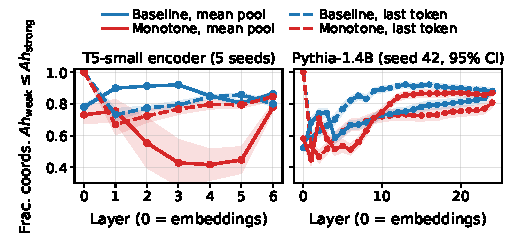
\includegraphics[width=0.63\linewidth]{order_preservation_depth.pdf}
\caption{Order preservation along learned semantic directions versus depth. Left: T5-small encoder (mean $\pm$ s.d., five seeds). Right: Pythia-1.4B (MLP-both, seed 42; 95\% bootstrap CIs, 195 held-out pairs). Layer 0 is the embedding output; its last-token value is trivially 1 since all prompts share the final token.}
\label{fig:order}
\end{figure}

\subsection{Generalization to Decoder-Only Foundation Models}
\label{sec:results-pythia}
\textbf{Constraint scope.}
In the screening (Table~\ref{tab:pythia-variants}, Appendix~\ref{app:more-results}), constraining only the MLP input projection fails: perplexity rises 3.65-fold yet the HotFlip success rate \emph{rises} from 71.5\% to 83.5\%, suggesting that gradient signal routes around the constrained matrix through the unconstrained output projection and attention. Constraining both MLP projections (MLP-both, the T5 scope) reduces the success rate by 30.5 points; constraining the attention output projection instead of $W_{\mathrm{out}}$ (MLP-in + Attn-out) reduces it by 39.5 points at about double the perplexity penalty ($12.49\times$ vs.\ $6.80\times$), a diminishing return, so we select MLP-both.

\textbf{Multi-seed validation.}
Table~\ref{tab:pythia-seeds} reports MLP-both at full budget on three seeds. The HotFlip success rate falls from 69.0\% to 39.0--45.0\% (mean 42.5\%), a 26.5-point (38.4\% relative) reduction. Universal triggers, unlike on T5, substantially damage the decoder-only baseline (NLL $+16.1\%$) and the monotone models are less affected in relative terms ($+10.6\%$), but their clean NLL is roughly 1.9 times higher and the absolute increase is not smaller ($0.40 \pm 0.14$ vs.\ $0.32 \pm 0.01$ nats): monotonicity reduces the relative, but not the absolute, effect of triggers.

\begin{table}[t]
\caption{Pythia-1.4B, MLP-both, full budget. PPL: held-out Pile perplexity; SR: HotFlip success rate ($n = 200$, 10 flips, 15\% threshold); UAT: relative and absolute NLL increase under the trigger (base $\to$ mono).}
\label{tab:pythia-seeds}
\centering
\footnotesize
\begin{tabular}{lccccc}
\toprule
Seed & PPL base & PPL mono & SR base $\to$ mono & UAT NLL$\uparrow$ & UAT $\Delta$NLL (nats) \\
\midrule
42   & 6.72 & 36.01 & 69.0\% $\to$ 43.5\% & $+15.5\% \to +8.8\%$ & $0.31 \to 0.33$ \\
1337 & 6.72 & 42.00 & 69.0\% $\to$ 39.0\% & $+16.4\% \to +8.1\%$ & $0.33 \to 0.32$ \\
2024 & 6.72 & 35.03 & 69.0\% $\to$ 45.0\% & $+16.5\% \to +15.0\%$ & $0.33 \to 0.56$ \\
\midrule
Mean & 6.72 & 37.68 & 69.0\% $\to$ 42.5\% & $+16.1\% \to +10.6\%$ & $0.32 \to 0.40$ \\
\bottomrule
\end{tabular}
\end{table}

\textbf{Transfer and gradient-free controls.}
Table~\ref{tab:pythia-controls} reports the controls of Section~\ref{sec:setup-pythia}, which address the concern that a constrained model merely masks gradients~\citep{athalye2018obfuscated,carlini2019evaluating,tramer2020adaptive}. First, the monotone model's advantage persists under every gradient-free attack (random substitutions degrade the baseline by 64.6 percent vs.\ 17.9 percent for the monotone model; the query attack by 112 vs.\ 34 percent); since neither uses gradients, the gap cannot be gradient masking. Second, attacks do not transfer symmetrically: substitutions crafted on the baseline degrade the monotone model by only 15.4 percent, less than random ones, whereas substitutions crafted on the monotone model degrade the baseline by 65.0 percent, as much as random ones (triggers behave the same way; Appendix~\ref{app:transfer}). Third, absolute gaps are narrower (random 0.66 vs.\ 0.91 nats; query 1.17 vs.\ 1.39; HotFlip 0.77 vs.\ 0.82) because the monotone model's clean NLL is roughly 1.9 times higher: it is less sensitive to every substitution type tested, but part of its relative advantage reflects its higher clean loss, a caveat far weaker for T5 (absolute gap 2.5-fold).

\begin{table}[t]
\caption{Transfer and gradient-free controls on Pythia-1.4B (MLP-both, full budget; mean $\pm$ s.d.\ over three seeds; 10 substitutions on 200 held-out texts, query attack on 50). Deg.: mean relative loss increase; SR: success rate (15\% threshold); $\Delta$NLL: absolute increase (nats). HotFlip rows re-run Table~\ref{tab:pythia-seeds}'s attack inside the transfer pipeline.}
\label{tab:pythia-controls}
\centering
\footnotesize
\setlength{\tabcolsep}{2pt}
\begin{tabular}{llcccccc}
\toprule
 & & \multicolumn{3}{c}{Evaluated on baseline} & \multicolumn{3}{c}{Evaluated on monotone} \\
\cmidrule(lr){3-5}\cmidrule(lr){6-8}
Attack & Crafted on & Deg. & SR & $\Delta$NLL & Deg. & SR & $\Delta$NLL \\
\midrule
HotFlip & baseline & $55.2 \pm 0.4\%$ & $68.7 \pm 0.3\%$ & 0.82 & $15.4 \pm 1.3\%$ & $25.8 \pm 1.6\%$ & 0.57 \\
HotFlip & monotone & $65.0 \pm 0.9\%$ & $72.8 \pm 1.8\%$ & 0.94 & $20.5 \pm 1.6\%$ & $42.5 \pm 3.1\%$ & 0.77 \\
Random substitutions & --- & $64.6 \pm 0.3\%$ & $73.0 \pm 1.0\%$ & 0.91 & $17.9 \pm 1.5\%$ & $36.5 \pm 2.3\%$ & 0.66 \\
Query (gradient-free) & target & $112.3 \pm 4.0\%$ & $77.3 \pm 1.2\%$ & 1.39 & $33.6 \pm 2.9\%$ & $50.0 \pm 3.5\%$ & 1.17 \\
\bottomrule
\end{tabular}
\end{table}

\textbf{The quality--robustness trade-off is architecture-dependent.}
Monotonicity is not universally ``free'': held-out perplexity of the monotone Pythia model is 5.61$\times$ that of its baseline even after full-budget recovery training, whereas the T5 monotone model's validation perplexity is only about $1.35\times$ its baseline's with ROUGE-L within 5\%. We conjecture an architectural explanation: in a decoder-only block the constrained FFN must absorb a larger share of the block's transformation, whereas T5's encoder--decoder bottleneck and cross-attention carry more of it unconstrained and also restrict the routes by which perturbations bypass constrained sublayers.

\section{Discussion and Conclusion}
\label{sec:discussion}
This work provides empirical evidence, and a conditional theoretical mechanism, that monotonicity is a promising architectural bias for language-model robustness: enforcing it in feed-forward sublayers consistently reduces vulnerability to token-level attacks while largely preserving task performance in encoder--decoder models. The gradient-free Pythia-1.4B controls show that the advantage is not confined to gradient-based attacks, so the mechanism of Section~\ref{sec:gradient-attenuation} is one facet of a more general reduction in sensitivity to token-level perturbations rather than gradient masking. The order-preservation diagnostic shows that per-sublayer, coordinatewise monotonicity does not itself make the network more order-preserving along learned semantic directions: that ordering (Section~\ref{sec:intro}) is the design principle, whereas the experiments support a local sensitivity reduction in the constrained sublayers; imposing the constraint in a learned semantic basis $A$ is a natural next step (see Appendix~\ref{app:discussion}).

Our study is limited to modest model scales, provides no formal certificates, and leaves open whether the robustness gain, like the clean-quality cost, is attributable to the initialization rather than the constraint (Appendix~\ref{app:ablation}). Consistent improvements across two Transformer families nevertheless suggest that monotonicity is a principled architectural prior for robust language models at an architecture-dependent cost in clean performance.

\subsection*{AI use statement}
Generative AI tools (Anthropic's Claude, via Claude Code) were used in this work to help develop and debug the experiment pipeline that implements the method and attacks, to compute, from the raw per-seed outputs, the aggregate statistics reported in the tables and to draft their interpretation, and to check and correct the statements and proofs of Section~\ref{sec:gradient-attenuation} and Appendix~\ref{app:proofs}; the corrected statements were re-derived and verified by the authors, and every reported number was recomputed by the authors from the raw outputs. Generative AI tools were not used to generate synthetic data or to propose the hypotheses or the research methodology, and no experiment was designed, run, or altered by an AI tool; the remaining required-disclosure categories of the ICLR policy are not applicable to this work. AI tools were also used to draft and edit parts of the text for readability, to identify and verify related literature and format references, and to produce Figure~\ref{fig:order} from the experimental outputs. All AI-assisted code was tested by the authors, all AI-suggested references were checked against their primary sources, and all AI-assisted text and mathematics were reviewed by the authors. We take responsibility for the final content of this work, including text, claims, and artifacts produced with the aid of generative AI.

\subsection*{Ethics statement}
This work explores architectural constraints that improve the robustness of language models to adversarial manipulation. By studying monotonicity as a structural inductive bias, our approach contributes to the development of language models whose behavior is more predictable and analyzable, which is particularly relevant for safety-critical and decision-support applications. All experiments use publicly available pretrained models (T5-small, Pythia-1.4B) and public datasets; no human subjects or private data are involved. The attacks studied are standard, previously published token-level attacks evaluated on summarization and language-modeling loss, and do not produce new capabilities for misuse.

\subsection*{Reproducibility statement}
Sections~\ref{Prelim} and~\ref{sec:setup} state the method as implemented (the coordinatewise instantiation, the softplus reparameterization, and the initialization), and Appendix~\ref{app:training}, Appendix~\ref{app:seeds}, and Appendix~\ref{app:pythia} give the complete training, evaluation, attack, and hardware settings for both tracks, including the seeds, the statistical tests, and the precision used at each stage. All theoretical statements are proved in Appendices~\ref{app:model-details}, \ref{app:proofs}, and~\ref{app:mechanism-details}, with their assumptions stated explicitly. Every multi-seed entry in the tables is a mean (and, where shown, standard deviation) over the per-seed result files, as described in Appendix~\ref{app:seeds}; Tables~\ref{tab:hotflip}, \ref{tab:pythia-variants}, and \ref{tab:ablation} report single seeds, as stated in their captions.
The code for the full pipeline (training, attacks, controls, and the order-preservation probe) and the per-seed result files will be released with the camera-ready version.

\bibliography{example_paper}
\bibliographystyle{iclr2027_conference}


%%%%%%%%%%%%%%%%%%%%%%%%%%%%%%%%%%%%%%%%%%%%%%%%%%%%%%%%%%%%%%%%%%%%%%%%%%%%%%%
%%%%%%%%%%%%%%%%%%%%%%%%%%%%%%%%%%%%%%%%%%%%%%%%%%%%%%%%%%%%%%%%%%%%%%%%%%%%%%%
% APPENDIX
%%%%%%%%%%%%%%%%%%%%%%%%%%%%%%%%%%%%%%%%%%%%%%%%%%%%%%%%%%%%%%%%%%%%%%%%%%%%%%%
%%%%%%%%%%%%%%%%%%%%%%%%%%%%%%%%%%%%%%%%%%%%%%%%%%%%%%%%%%%%%%%%%%%%%%%%%%%%%%%
\newpage
\appendix
\section{Appendix}
\label{app:top}



% \subsection{Related Work}

\subsection{Extended Related Work}
\label{app:related}

\textbf{Vulnerabilities of Language Models.}
Large language models are highly susceptible to adversarial manipulations that bypass alignment and safety mechanisms. Prior work has documented jailbreak prompts and transferable adversarial suffixes that generalize across models and settings, including aligned systems~\citep{Zou2023UniversalTransferableAttacksOnAlignedLLMs}. Subsequent studies identify additional failure modes, such as position-sensitive jailbreaks~\citep{wang2025vulnerability}, interpretable attacks that evade perplexity-based defenses~\citep{Zhu2023AutoDAN}, and many-shot jailbreaks whose effectiveness increases with larger context windows~\citep{anil2024many}. Robustness benchmarks further show that models perform poorly under systematic adversarial evaluation~\citep{Wang2021AdvGLUE}, and that safety mechanisms often fail in multilingual or low-resource settings~\citep{deng2024multilingual}. Prompt injection attacks, which exploit the lack of separation between instruction and context, are now recognized as a fundamental vulnerability, alongside broader threats to inference and training-time surveyed in recent security analyses~\citep{li2025security}.
At the token level, the attacks we use descend from a well-developed lineage: gradient-guided substitutions~\citep{ebrahimi2018hotflip}, universal triggers~\citep{wallace2019universal}, and their prompt-search descendants~\citep{shin2020autoprompt}; fully gradient-based relaxations for Transformers~\citep{guo2021gradient}; gradient-free, query-based word substitutions~\citep{jin2020bert}; and attacks designed specifically for sequence-to-sequence models~\citep{cheng2020seq2sick}.

\textbf{Defenses and Robustness Enhancements.}
Proposed defenses include smoothing-based methods with provable jailbreak guarantees~\citep{Robey2023SmoothLLM},
prompt-level classifiers trained on synthetic jailbreak data~\citep{sayeedi2025jailbreaktracer}, and adversarial training approaches whose effectiveness depends on model scale and threat model~\citep{howe2024effects}.
Adversarial prompts also transfer across models, so that a defense evaluated against a single attacker can be circumvented by suffixes optimized elsewhere~\citep{Zou2023UniversalTransferableAttacksOnAlignedLLMs}.
Simple input-side baselines such as perplexity filtering and paraphrasing are surprisingly competitive against optimization-based attacks~\citep{jain2023baseline}, representation-level interventions reroute the internal activations responsible for harmful outputs~\citep{zou2024circuit}, and certified training bounds the effect of word substitutions for small classifiers~\citep{jia2019certified}. Despite these advances, most defenses remain reactive and training-dependent. A recurring lesson from the vision literature is that apparent robustness to gradient-based attacks can be an artifact of obfuscated gradients, so that any architectural defense must be evaluated with gradient-free and adaptive attacks as well~\citep{athalye2018obfuscated,carlini2019evaluating,tramer2020adaptive}; the random-substitution and query-based controls of Section~\ref{sec:results-pythia} follow this guidance.

\textbf{Monotonic Neural Networks and Structural Constraints.}
Monotonicity has long been studied as a structural inductive bias for interpretability and robustness. Classical results show that feed-forward networks with non-negative weights and sigmoidal activations~\citep{Daniels2010Monotone}, as well as min--max networks of sign-constrained linear units~\citep{Sill1998MonotonicNetworks}, are universal approximators of monotone functions, establishing that monotonicity need not limit expressivity. Subsequent work proposed practical monotone and partially monotone architectures, including lattice-based models, enabling scalable learning under monotonic constraints in structured domains~\citep{Gupta2016MonotonicLattices,You2017DeepLattice}. More recent work certifies monotonicity of piecewise-linear networks by mixed-integer linear programming~\citep{liu2020certified} or counterexample-guided repair~\citep{sivaraman2020counterexample}.
Alternatives to sign-constrained weights include integrating a positive derivative network~\citep{wehenkel2019unconstrained}, smooth min--max constructions~\citep{igel2024smooth}, and Lipschitz-bounded residual architectures that are monotone by construction and simultaneously certify robustness~\citep{nolte2023expressive,kitouni2023robust}; the price of the nonnegative-parameter inductive bias in depth and width has been characterized theoretically~\citep{mikulincer2022size}, and nonnegative weight constraints have also been used for interpretability in multilayer perceptrons~\citep{chorowski2015learning}. The observation that monotone classifiers are structurally resistant to a class of evasion attacks predates the LLM era~\citep{incer2018adversarially}. In control theory, monotone (cooperative) systems admit order-preserving flows with strong convergence properties~\citep{hirsch2006monotone,angeli2003monotone}, and structural order can, under suitable conditions, reduce verification to extremal cases~\citep{feyzmahdavian2017stability}, an intuition we draw on in Section~\ref{sec:gradient-attenuation}; monotone operator theory has separately been used to guarantee well-posedness of implicit-depth networks~\citep{winston2020monotone}. More broadly, architectural constraints and structured layers have been shown to improve robustness and stability without prohibitive performance loss~\citep{Amos2017OptNet}, and controlling the Lipschitz constant of attention has been proposed as a structural route to more stable Transformers~\citep{kim2021lipschitz,newhouse2025training}. Our work builds on this line by showing that selectively enforced monotonicity can scale to Transformer-based language models and yield tangible robustness gains.


\subsection{Additional Details on the Monotone Transformer}
\label{app:model-details}
\begin{proof}[Proof of Proposition~\ref{prop:amono}]
If $Ah \le Ah'$, monotonicity of $g$ gives $g(Ah) \le g(Ah')$, and
\begin{align*}
A F(h)
&= Ah + A A^\dagger g(Ah) \\
&= Ah + g(Ah) \\
&\le Ah' + g(Ah') \\
&= A F(h').
\end{align*}

\end{proof}

Note that $\preceq$ is a preorder rather than a partial order whenever $p < d$: $h \preceq h' \preceq h$ holds exactly when $h - h' \in \ker(A)$, and such pairs are indistinguishable to the constraint; when $A = I$, $\preceq$ is the coordinatewise partial order.

\begin{remark}[Placement inside a pre-normalized block]
\label{rem:preln}
In the T5 and GPT-NeoX blocks we instantiate (with $A = I$), the FFN branch receives the normalized residual state $u = \mathrm{LN}(h)$, where $\mathrm{LN}$ denotes the block's normalization layer, and the residual connection is applied outside the branch, $F(h) = h + g(\mathrm{LN}(h))$, with $g(u) = W_{\mathrm{o}}\,\mathrm{ReLU}(W_{\mathrm{i}} u)$ in T5 (no biases) and $g(u) = W_{\mathrm{out}}\,\mathrm{GELU}(W_{\mathrm{in}} u + b_{\mathrm{in}}) + b_{\mathrm{out}}$ in GPT-NeoX. The normalization (a root-mean-square rescaling with an unconstrained gain in T5; standard layer normalization with mean centering, gain, and bias in GPT-NeoX) is not monotone, so $F$ need not be coordinatewise monotone as a map of $h$. The property we enforce, and the object of the analysis in Section~\ref{sec:gradient-attenuation}, is the monotonicity of the branch $g$ as a map of its own input $u$; the residual path is the identity and is unaffected by the constraint.
\end{remark}

\subsection{Mathematical Proofs}
\label{app:proofs}
\subsubsection{Proof of Lemma~\ref{lem:mono_comp}}
\label{prf:lem1}
\begin{proof}
For any $x, x' \in \mathbb{R}^n$ such that $x \le x'$, monotonicity of $f$ implies $f(x) \le f(x')$. Applying monotonicity of $g$ yields
\[
g(f(x)) \le g(f(x')),
\]
which establishes the claim.
\end{proof}

\subsubsection{Proof of Lemma~\ref{lem:jacobian-nonneg}}

\label{prf:jac}
\begin{proof}
Recall $T(s)=s+g(s)$, so at every point of differentiability
\[
J_T(s)=\partial T(s)/\partial s=I + J_g(s).
\]
For a two-layer $g(s)=W_2 \sigma(W_1 s + b_1)+b_2$ with $W_1,W_2\ge 0$ elementwise,
\[
J_g(s)=W_2 \operatorname{diag}(\sigma'(W_1 s + b_1)) W_1.
\]
Since $\sigma$ is elementwise non-decreasing, $\sigma'(z)\ge 0$ wherever it exists,
so $\operatorname{diag}(\sigma'(\cdot))\ge 0$ elementwise. Hence $J_g(s)\ge 0$
elementwise, and therefore $J_T(s)=I+J_g(s)\ge 0$ elementwise.
For an $L$-layer $g$ with hidden states $h_\ell = \sigma(z_\ell)$ and pre-activations
$z_\ell = W_\ell h_{\ell-1} + b_\ell$ (with $h_0 = s$),
\[
J_g(s)=W_L\,\operatorname{diag}(\sigma'(z_{L-1}))\,W_{L-1}\,\operatorname{diag}(\sigma'(z_{L-2}))\cdots W_2\,\operatorname{diag}(\sigma'(z_1))\,W_1
\]
is a product of
$L$ weight matrices and $L-1$ diagonal matrices, each elementwise nonnegative, and is
therefore elementwise nonnegative, so the conclusion is unchanged. At a point $s$ where
some pre-activation lies at a kink of $\sigma$ (for ReLU, $z_j = 0$), $T$ is locally
Lipschitz whenever $\sigma$ is, and its Clarke generalized Jacobian is by definition the
convex hull of all limits $\lim_k J_T(s_k)$ along sequences $s_k \to s$ of points of
differentiability. Each $J_T(s_k)$ is elementwise nonnegative by the product formula,
and the set of elementwise nonnegative matrices is closed and convex, so every element
of the Clarke generalized Jacobian is elementwise nonnegative. Reverse-mode automatic
differentiation evaluates the same product with $\sigma'(z_j)$ at a kink replaced by the
framework's convention (for ReLU in PyTorch, $\sigma'(0)=0$); for any nonnegative
convention the result is again a product of nonnegative matrices.
\end{proof}

\subsubsection{Proof of Lemma~\ref{lem:gradient-attenuation}}
\label{prf:atten}
\begin{proof}
Write $D(s) := \operatorname{diag}(\sigma'(z(s)))$. Then
$J_g(s) = W_2 D(s) W_1 = \sum_{j=1}^m \sigma'(z_j(s))\, W_2[:,j]\, W_1[j,:]$, which is
the stated decomposition. With $v := \nabla_{s'}\mathcal{L}$,
\[
\nabla_s \mathcal{L}(T(s)) = (I + J_g(s))^\top v
= v + \sum_{j=1}^m \sigma'(z_j(s))\, W_1[j,:]^\top \bigl(W_2[:,j]^\top v\bigr).
\]
Splitting the sum into $j \in S$ and $j \notin S$, the difference in the statement
equals $\sum_{j\in S} \sigma'(z_j(s))\, W_1[j,:]^\top (W_2[:,j]^\top v)$. By the
triangle and Cauchy--Schwarz inequalities its Euclidean norm is at most
\[
\sum_{j\in S} |\sigma'(z_j(s))|\, \|W_1[j,:]\|_2\, \|W_2[:,j]\|_2\, \|v\|_2
\;\le\; \varepsilon\, G \sum_{j\in S} \|W_2[:,j]\|_2\, \|W_1[j,:]\|_2 .
\]
For the final claim, if $z_j(s_k) \to -\infty$ for all $j \in S$ then
$\max_{j\in S}|\sigma'(z_j(s_k))| \to 0$ by Assumption~\ref{ass:saturation}, so
the bound above tends to $0$ as long as $\|\nabla_{s'}\mathcal{L}\|_2$ stays bounded
along the sequence.
\end{proof}



\subsection{Gradient Attenuation: Full Derivations and Discussion}
\label{app:mechanism-details}
This appendix reproduces the complete text of the mechanism analysis, including the chain-rule decomposition, the discussion of sign coherence, and the scope of the analysis.

We propose a candidate mechanism for the empirical robustness gains observed in monotone Transformer language models.
Rather than claiming global robustness guarantees, we analyze how monotonicity constraints alter the local gradient structure of feed-forward sublayers in a way that can reduce the effectiveness of gradient-based adversarial attacks such as HotFlip.

Our analysis is motivated by classical results in the theory of monotone dynamical systems, which show that, for strongly monotone (cooperative and irreducible) flows, almost every bounded trajectory converges to the set of equilibria~\citep{hirsch1985systems}.
While a feed-forward network is not a time-indexed dynamical system in this sense, and convergence of states says nothing directly about input--output sensitivities, this perspective suggests that monotonicity can limit the set of active directions along which outputs and gradients vary. We leverage this intuition to inform a local analysis of gradient behavior under monotone perturbations, focusing on how saturation and non-negative weights interact to diminish exploitable gradient directions.

Consider an $A$-monotone FFN update
\[
F(h) := h + A^\dagger\, g(Ah),
\]
where $A\in\mathbb{R}^{p\times d}$ is fixed, $A^\dagger$ satisfies $AA^\dagger=I_p$,
and $g:\mathbb{R}^p\to\mathbb{R}^p$ is coordinatewise monotone (e.g., an MLP with
elementwise non-decreasing activations and elementwise nonnegative weight matrices).
Let $s := Ah \in \mathbb{R}^p$ denote semantic coordinates and define the induced
semantic refinement map
\[
T(s) := A F(h) = s + g(s).
\]
We analyze the Jacobian of $T$ and its implications for gradients with respect to
semantic coordinates. (In general, $J_F(h)$ need not be elementwise nonnegative in
$\mathbb{R}^d$ due to $A^\dagger$.)
In our experiments $A = I$, and we take as $s$ the input $u = \mathrm{LN}(h)$ of the FFN branch of
Remark~\ref{rem:preln}, with $g$ the branch itself. Because the block is
pre-normalized, the residual adds $h$ rather than $s$, so $T$ is not literally the
sublayer map $h \mapsto F(h) = h + g(\mathrm{LN}(h))$, whose Jacobian is
$I_d + J_g(\mathrm{LN}(h))\,J_{\mathrm{LN}}(h)$; for the trained models the chain-rule
decomposition below therefore holds with the correction term multiplied on the left by
the unconstrained factor $J_{\mathrm{LN}}(h)^{\top}$. All statements that follow concern
the branch factor $J_g$ and are unaffected by this factor.

% \subsubsection{Preliminaries}

% Consider a feed-forward sublayer $f : \mathbb{R}^d \to \mathbb{R}^d$ of the form
% \begin{equation}
% f(x) = W_2 \sigma(W_1 x + b_1) + b_2,
% \end{equation}
% where $W_1, W_2 \in \mathbb{R}^{d \times d}$ have non-negative entries and
% $\sigma$ is an elementwise, monotone non-decreasing activation function
% (e.g., ReLU or softplus). Under these conditions, $f$ is monotone with respect
% to the standard partial order on $\mathbb{R}^d$.

% We study the Jacobian structure of $f$ and its implications for gradients
% of a scalar loss function $L(f(x))$ with respect to the input $x$.

% \subsubsection{Jacobian Structure of Monotone Sublayers}

\begin{lemmastar}[Lemma~\ref{lem:jacobian-nonneg}, full statement]
Let $g$ be an MLP with elementwise non-decreasing activation $\sigma$ and
elementwise nonnegative weight matrices. At every $s \in \mathbb{R}^p$ at which $g$
is differentiable (all $s$ if $\sigma$ is continuously differentiable;
Lebesgue-almost every $s$ for ReLU), the Jacobian
\[
J_T(s) = \partial T(s)/\partial s = I + J_g(s)
\]
has non-negative entries. The same holds for every element of the Clarke
generalized Jacobian of $T$ (for locally Lipschitz $\sigma$), and likewise for the
matrix returned by reverse-mode automatic differentiation under any nonnegative
convention for $\sigma'$ at kinks.
\end{lemmastar}

This follows from $T(s)=s+g(s)$ and the factorization of the MLP Jacobian. For a
two-layer $g(s)=W_2\sigma(W_1 s + b_1)+b_2$ with $W_1,W_2\ge 0$ elementwise,
\[
J_g(s)=W_2\,\mathrm{diag}(\sigma'(W_1 s+b_1))\,W_1 \ge 0 \quad (\text{elementwise}),
\]
hence $J_T(s)=I + J_g(s)\ge 0$ elementwise; for deeper $g$ the Jacobian is a product
of elementwise nonnegative matrices (Appendix~\ref{prf:jac}).
Intuitively, increasing any semantic coordinate cannot decrease any output semantic
coordinate through $T$; sign cancellations are ruled out \emph{within semantic space}.

Let $\ell:\mathbb{R}^d\to\mathbb{R}$ be the differentiable objective induced by the
rest of the network on the sublayer output $h' = F(h)$. Since
$J_F(h) = I_d + A^\dagger J_g(Ah)\, A$, the chain rule gives
\[
\nabla_h\, \ell(F(h)) \;=\; \nabla \ell(h') \;+\; A^{\top} J_g(Ah)^{\top} (A^\dagger)^{\top} \nabla \ell(h').
\]
The first term is the residual path and is unaffected by the constraint; the second
is a correction of rank at most $p$ that acts, through $J_g^\top$, on the downstream
gradient expressed in semantic coordinates, $v := (A^\dagger)^{\top}\nabla \ell(h')
\in \mathbb{R}^p$. For brevity we write $\nabla_{s'}\mathcal{L} := v$; the
semantic-space gradient on which the constraint acts is then
\[
\nabla_s \mathcal{L}(T(s)) \;:=\; J_T(s)^\top \nabla_{s'} \mathcal{L}
\;=\; \nabla_{s'}\mathcal{L} + J_g(s)^\top \nabla_{s'}\mathcal{L}.
\]
Thus the backpropagated gradient in semantic space equals the residual-path gradient
plus an additive correction whose matrix has nonnegative entries under
Lemma~\ref{lem:jacobian-nonneg}. Nonnegativity rules out sign cancellation inside
this correction; it does not by itself reduce its magnitude (indeed $J_T \ge I$
elementwise). All statements below concern this correction term.


\subsubsection{Saturation-Induced Gradient Attenuation}
We now examine how saturation in monotone networks affects gradient magnitude. The idea is simple: a hidden unit whose activation is flat at its current pre-activation contributes nothing to the gradient that flows through it, so the more units sit in such a flat regime, the fewer directions an attacker can exploit. The assumption below fixes what ``flat'' means for the activations we use, and the lemma quantifies the contribution of nearly flat units.
\begin{assumptionstar}[Assumption~\ref{ass:saturation}, restated]
The activation $\sigma$ used inside $g$ has bounded derivative and admits a
saturated regime in the negative direction: $|\sigma'(z)| \to 0$ as $z\to -\infty$,
and $|\sigma'|$ is non-decreasing on some tail $(-\infty, z^\ast]$. This holds exactly
for ReLU, used by T5-small ($\sigma'(z) = 0$ for all $z < 0$, with $z^\ast = 0$), and
for the softplus and logistic activations (with any $z^\ast \le 0$); GELU, used by Pythia,
satisfies it with $z^\ast = -\sqrt{2}$. ReLU, softplus, and GELU do not saturate in the positive direction, where
$\sigma'(z) \to 1$; the logistic activation saturates on both tails, but only
negative-tail saturation is used below.
\end{assumptionstar}



\begin{lemmastar}[Lemma~\ref{lem:gradient-attenuation}, restated]
Let $T(s)=s+g(s)$ with $g(s)=W_2\sigma(W_1 s+b_1)+b_2$, $W_1\in\mathbb{R}^{m\times p}$
and $W_2\in\mathbb{R}^{p\times m}$ elementwise nonnegative, and write
$z_j(s) := (W_1 s + b_1)_j$. Wherever $\sigma$ is differentiable at $z(s)$,
\[
J_g(s) = \sum_{j=1}^{m} \sigma'(z_j(s))\, W_2[:,j]\, W_1[j,:],
\]
so that each hidden unit contributes a rank-one term to $J_g$ weighted by its
derivative. Let $S \subseteq \{1,\dots,m\}$ be a set of units with
$\max_{j\in S} |\sigma'(z_j(s))| \le \varepsilon$, and suppose
$\|\nabla_{s'}\mathcal{L}\|_2 \le G$. Then
\[
\Big\| \nabla_s \mathcal{L}(T(s)) - \Big( I + \sum_{j\notin S} \sigma'(z_j(s))\, W_2[:,j]\, W_1[j,:] \Big)^{\!\top} \nabla_{s'}\mathcal{L} \Big\|_2
\;\le\; \varepsilon\, G \sum_{j\in S} \|W_2[:,j]\|_2\, \|W_1[j,:]\|_2 .
\]
In particular, if $\sigma$ satisfies Assumption~\ref{ass:saturation}, then along any
sequence $\{s_k\}$ on which the pre-activations of the units in $S$ diverge to
$-\infty$ while $\nabla_{s'}\mathcal{L}$ remains bounded,
the contribution of those units to $J_g(s_k)$, and hence to
$\nabla_s \mathcal{L}(T(s_k))$, vanishes.
\end{lemmastar}


The proof is given in Appendix~\ref{prf:atten}.

This result shows that activation saturation can locally suppress the feed-forward
branch's own contribution $J_g^\top\nabla_{s'}\mathcal{L}$ to the backpropagated
gradient, driving the sublayer Jacobian toward the identity of the residual path,
without eliminating all gradient signal. Nonnegativity of the weights is not needed
for the bound itself; its role is to prevent cancellation among the remaining active
units (Lemma~\ref{lem:jacobian-nonneg}). Because of this, the suppression is a
genuine attenuation whenever the downstream gradient is sign-coherent: if
$\sigma' \ge 0$ and $\nabla_{s'}\mathcal{L} \ge 0$ (or $\le 0$) elementwise, every
coordinate of $\nabla_{s'}\mathcal{L} + J_g^\top\nabla_{s'}\mathcal{L}$ is
non-decreasing in absolute value in each $\sigma'(z_j)$, so saturating units can
only shrink $\|\nabla_s\mathcal{L}(T(s))\|$ toward $\|\nabla_{s'}\mathcal{L}\|$.
The condition $\sigma' \ge 0$ holds everywhere for ReLU, but for GELU it fails
precisely on the saturated tail ($\mathrm{GELU}'(z) < 0$ for $z < -0.752$), so this
monotone-attenuation reading applies to the T5 track, while for the Pythia track only
the norm bound of Lemma~\ref{lem:gradient-attenuation} is available. For mixed-sign
downstream gradients, removing a unit's contribution can increase the norm, and the
lemma should be read as a statement about the feed-forward term alone.


\subsubsection{Persistence of Saturation Effects}

The following observation captures a one-sided stability property of saturated
units under monotone perturbations.

\begin{lemma}[Persistence of Saturated Units]
\label{lem:persistence}
Let $\sigma$ satisfy Assumption~\ref{ass:saturation} with tail threshold $z^\ast$,
and consider any first-layer pre-activation $z_j(s)= (W_1 s + b_1)_j$ within $g$,
with $W_1\ge 0$ elementwise. For $\varepsilon \ge 0$, call unit $j$
\emph{$\varepsilon$-saturated} at $s$ if $z_j(s) \le z^\ast$ and
$|\sigma'(z_j(s))| \le \varepsilon$ (for ReLU, with the convention $\sigma'(0)=0$,
$0$-saturated means $z_j(s) \le 0$). If unit $j$ is $\varepsilon$-saturated at $s'$,
then for any monotone semantic perturbation $\delta \le 0$, i.e., for any
$s' + \delta \le s'$ in the product order on $\mathbb{R}^p$, the unit remains
$\varepsilon$-saturated at $s'+\delta$.
\end{lemma}

\label{prf:persis}
\begin{proof}
Let $z_j(s) := (W_1 s + b_1)_j$. Since $W_1\ge 0$ elementwise and $\delta\le 0$,
\[
z_j(s' + \delta) = z_j(s') + (W_1 \delta)_j \le z_j(s') \le z^\ast .
\]
Because $|\sigma'|$ is non-decreasing on $(-\infty, z^\ast]$ by
Assumption~\ref{ass:saturation}, $|\sigma'(z_j(s'+\delta))| \le |\sigma'(z_j(s'))|
\le \varepsilon$. Thus the unit remains $\varepsilon$-saturated at $s'+\delta$.
For ReLU with $z^\ast = 0$ the argument is simply that $z_j(s') \le 0$ implies
$z_j(s'+\delta) \le 0$.
\end{proof}

Importantly, this lemma applies to individual hidden units rather than to the
entire input gradient, and does not preclude other units from becoming active.
Its
direction is set by the activation: for the activations used here, saturation is
preserved under monotone decreases of the semantic coordinates, whereas a monotone
increase can re-activate a saturated unit.
\subsubsection{Implications for Gradient-Based Attacks}

Gradient-based adversarial attacks such as HotFlip rely on persistent,
high-magnitude gradients with respect to token embeddings to identify impactful
discrete perturbations. The preceding analysis is conditional: it does not show
that the constraint \emph{produces} saturation, and whether training under
nonnegativity places pre-activations of $g$ in saturated regimes is an empirical
question that we do not test here. What it shows is that, \emph{if} hidden units
of $g$ are saturated, their contribution to the semantic gradient is small
(Lemma~\ref{lem:gradient-attenuation}), that this state is stable under monotone
decreases of the semantic coordinates (Lemma~\ref{lem:persistence}), and that the
contributions of the remaining active units cannot cancel one another
(Lemma~\ref{lem:jacobian-nonneg}; this last property requires $\sigma' \ge 0$ and
therefore holds exactly for the ReLU FFNs of the T5 track and only up to the small
negative-derivative region of GELU for the Pythia track). Together these properties
reduce the number and the variability of the directions through which a
gradient-based attacker can move the sublayer output.

\textbf{Scope.} The analysis concerns the feed-forward branch of a single sublayer.
The gradient with respect to token embeddings that HotFlip uses is a product of
Jacobians across all sublayers, in which the residual identity, attention, and
normalization paths are unconstrained; even if every feed-forward correction term
vanished, this product would reduce to that of the unconstrained paths. The
mechanism is therefore local, and the controls of Section~\ref{sec:results-pythia}
(random and gradient-free attacks) are needed to establish that the observed
robustness is not an artifact of gradient-based optimization.

While monotone feed-forward networks are not dynamical systems in the formal
sense, their behavior is reminiscent of classical results in monotone dynamical
systems, where cooperative interactions restrict the effective directions along
which trajectories evolve. This analogy is intended as intuition rather than a
formal guarantee: monotonicity does not prevent all adversarial attacks, nor do
gradients vanish globally. Instead, our analysis identifies a local attenuation
effect that weakens gradient-based optimization strategies, offering a plausible
mechanism for the empirical robustness improvements observed in
Section~\ref{sec:results}.




\subsection{Training and Evaluation Protocol}
\label{app:training}
Both baseline and monotone models are fine-tuned from the same pretrained \texttt{T5-small} checkpoint under identical optimization settings. We use the AdamW optimizer with learning rate $5 \times 10^{-5}$ and weight decay $0.01$, a batch size of 4, and gradient clipping with norm 1.0. To accommodate the constrained parameterization, the monotone model employs an extended warmup phase of 15\% of training steps, compared to 10\% for the baseline; we did not ablate this choice. Both models are trained for 7 epochs with linear learning-rate decay after warmup and receive the same total training budget; the checkpoint with the lowest validation loss is used for all downstream evaluation.

Training is conducted on the DialogSum, HighlightSum, and arXiv abstract datasets, comprising 242{,}774 examples in total, with 8{,}296 validation examples drawn from the corresponding validation splits.
Evaluation is performed on two held-out benchmarks using their full test sets: CNN/DailyMail (11{,}490 test examples) and XSUM (11{,}333 test examples; one example with an empty field is dropped by the loader).
Neither CNN/DailyMail nor XSUM is used in training, so both evaluations measure out-of-distribution generalization.

At inference time, decoding is performed using beam search with 4 beams and a length penalty of 1.2, enforcing a minimum generation length of 10 tokens and a maximum length of 80 tokens. We additionally apply no-repeat $n$-gram blocking with $n=3$ to discourage degenerate repetitions. All decoding parameters are fixed across models and evaluation sets.
ROUGE-1, ROUGE-2, and summary-level ROUGE-L (\texttt{rougeLsum}) F$_1$ scores are computed using the \texttt{rouge-score} library with Porter stemming. Within each seed we report bootstrap-based 95\% confidence intervals using 1{,}000 resamples and assess statistical significance via per-example paired $t$-tests between the baseline and monotone models, with Bonferroni correction across the three ROUGE variants. Effect sizes are reported using Cohen's $d$.

\subsection{Seeds, Statistical Tests, and Compute}
\label{app:seeds}
To evaluate robustness to training stochasticity, the T5 training and evaluation pipeline is repeated using five random seeds (42, 1337, 2024, 8888, and 12345), controlling randomness across Python, NumPy, and PyTorch. Summarization quality, training dynamics, and the order-preservation diagnostic are reported as the mean and standard deviation across all five seeds; universal-trigger attacks are reported across four seeds (1337, 2024, 8888, 12345; the seed-42 checkpoints were not evaluated under the final trigger protocol); the HotFlip evaluation in Table~\ref{tab:hotflip} uses the seed-2024 models, corroborated by an earlier evaluation of the seed-42 models.
Across-seed differences are assessed using paired $t$-tests on seed-level means (baseline vs.\ monotone ROUGE-L: $t = 14.9$ on CNN/DailyMail and $t = 13.4$ on XSUM with 4 degrees of freedom), complemented by per-example paired $t$-tests within each seed. This dual evaluation captures both test-time variability and variance induced by random initialization and data ordering. All experiments are conducted using deterministic algorithms where available, on NVIDIA A100 (40GB and 80GB), H200 (141GB), and RTX PRO 6000 (96GB) GPUs under the SLURM workload manager, using PyTorch builds with CUDA 11.8 (A100) or CUDA 12.8 (H200, RTX PRO 6000) and Transformers~4.30 or later.

\subsection{Foundation Model Training Protocol}
\label{app:pythia}
The decoder-only track fine-tunes Pythia-1.4B~\citep{biderman2023pythia} on the uncopyrighted subset of the Pile~\citep{gao2020pile}, with held-out evaluation texts drawn from a disjoint streaming sample. Constraint-scope screening (Table~\ref{tab:pythia-variants}) was run on seed 42, the MLP-in scope under the full budget described below and the MLP-both and MLP-in\,+\,Attn-out scopes under a reduced budget of 30{,}000 training samples at sequence length 1024 for 3 (baseline) and 4 (monotone) epochs; full-budget validation of the selected MLP-both scope (Table~\ref{tab:pythia-seeds}) trains the baseline for 5 epochs and the monotone model for 10 epochs on each of three seeds (42, 1337, 2024). The extended monotone budget parallels the extended warmup used in the T5 track and compensates for the constrained parameterization's slower recovery.
Both recovery runs use AdamW with weight decay $0.01$, linear warmup followed by linear decay, gradient clipping at norm $1.0$, an effective batch of 32 sequences (8 per step with 4 accumulation steps) at sequence length 2048, and bfloat16 weights with gradient checkpointing; the learning rate and warmup fraction are $10^{-5}$ and 10\% for the baseline and $5\times 10^{-5}$ and 20\% for the monotone model. Full-budget runs train on the first 100{,}000 documents of the streamed training split (90\%/10\% train/validation) and retain the checkpoint with the lowest validation perplexity. HotFlip evaluation uses 200 held-out examples with up to 10 token flips per example; UAT evaluation uses coordinate ascent with 3 restarts and 50 iterations, optimizing triggers on 80 texts and evaluating on 120 disjoint texts. Universal-trigger optimization and evaluation (including the trigger-transfer replay and the order-preservation probe) run with the models in bfloat16 precision; HotFlip, the substitution-transfer and gradient-free controls, and held-out perplexity are computed in float32.
All foundation-model experiments are executed on NVIDIA A100 GPUs with 80GB memory under the SLURM workload manager, with per-stage checkpointing to permit resumption across scheduler preemptions.

%%%%%%%%%%%%%%%%%%%%%%%%%%%%%%%%%%%%%%%%%%%%%%%%%%%%%%%%%%%%%%%%%%%%%%%%%%%%%%%
%%%%%%%%%%%%%%%%%%%%%%%%%%%%%%%%%%%%%%%%%%%%%%%%%%%%%%%%%%%%%%%%%%%%%%%%%%%%%%%


\subsection{Attack, Control, and Diagnostic Protocols}
\label{app:protocols}
This appendix reproduces the full protocol descriptions summarized in Section~\ref{sec:setup}.

\textbf{Universal Adversarial Triggers.}
Universal adversarial triggers (UATs)~\citep{wallace2019universal} consist of short, input-agnostic token sequences that, when prepended to an input, maximize the model's loss. We optimize five-token triggers using coordinate-wise search with five random restarts and 100 iterations.
Candidate tokens are drawn from a restricted pool of about 4{,}000 SentencePiece ids (ids 1000--4999) augmented with a short hand-picked list of negation and discourse words (e.g., \emph{not}, \emph{never}, \emph{ignore}), punctuation strings, and numerals; each iteration re-samples three of the five trigger positions, scores 50 random candidates per position on a random 30-example subset, and the trigger with the highest mean loss on the full optimization set is kept. Triggers are optimized on 1{,}000 held-out CNN/DailyMail validation examples and evaluated on 1{,}500 disjoint test examples; the cross-model transfer matrix is computed on the first 100 evaluation examples.
The trigger is inserted at the start of the encoder input, ahead of the \texttt{summarize:} prefix, and the concatenation is then truncated \emph{from the left} to the 512-token encoder budget. For articles longer than about 505 tokens the trigger is therefore partially or entirely discarded and the attacked input coincides with the clean input; because many CNN/DailyMail articles exceed this length, the universal-trigger results on T5 reflect only the shorter articles and should be read as a lower bound on trigger effectiveness.

\textbf{HotFlip Attacks.}
HotFlip attacks~\citep{ebrahimi2018hotflip} identify vulnerable input positions by computing gradients of the loss with respect to token embeddings and replacing selected tokens to maximize loss increase. We attack the five positions (special tokens excluded) with the largest gradient norms, selecting the replacement at each position by the dot product between the gradient and the candidate embedding.

\textbf{Robustness Metrics.}
Robustness is quantified using the relative increase in the model's cross-entropy loss under attack (\emph{degradation}, averaged over examples), the attack success rate (the fraction of examples whose degradation exceeds 10\%), and statistical significance assessed via independent-samples $t$-tests on the per-example degradations.
Because relative degradation is normalized by each model's own clean loss, we also report the absolute loss increase in nats, which is insensitive to differences in clean loss between models. For UATs we report the relative increase in negative log-likelihood (NLL) and ROUGE changes under the trigger, and analyze cross-model transferability of adversarial triggers.

\textbf{Order-preservation diagnostic.}
To test whether sublayer monotonicity translates into order preservation along the semantic directions that motivate it, we construct a templated corpus of ordered prompt pairs: 13 semantic axes (severity, safety constraints, certainty, urgency, and others, as in Section~\ref{sec:intro}) instantiated on 18 topics as four-level chains, yielding 702 adjacent-level pairs (weaker $\preceq$ stronger), split at the chain level into 507 probe-fitting and 195 disjoint evaluation pairs. For each model and pooling we fit $p=64$ probe directions $A$ on final-layer representations of the fitting split, each row being an $\ell_2$-regularized logistic-regression direction for stronger-versus-weaker fit on a bootstrap resample of the fitting pairs, so that the 64 rows are correlated readouts of one underlying ordering signal rather than 64 distinct axes. For every evaluation pair and every layer we then report the fraction of the $64$ probe coordinates for which $A h_{\mathrm{weak}} \le A h_{\mathrm{strong}}$, with bootstrap confidence intervals, under both mean and last-token pooling. This instrument is fit post hoc and plays no role in training.


\paragraph{Decoder-only track.}
The T5 experiments above concern an encoder-decoder architecture. To determine whether the monotonicity--robustness relationship generalizes to the decoder-only architectures that dominate contemporary foundation models, we conduct a second experimental track using Pythia-1.4B~\citep{biderman2023pythia}, a 24-layer autoregressive language model from the GPT-NeoX family. Models are fine-tuned and evaluated on the Pile~\citep{gao2020pile} (uncopyrighted subset), and clean performance is measured by \emph{perplexity}---the exponentiated mean negative log-likelihood per token---on a held-out sample, the standard intrinsic quality metric for autoregressive language models.

Because decoder-only blocks lack the encoder-decoder bottleneck of T5, it is not obvious which sublayers must be constrained for monotonicity to bind. Each GPT-NeoX block contains an attention sublayer with an output projection and a feed-forward (MLP) sublayer with an input projection ($W_{\mathrm{in}} \in \mathbb{R}^{4d \times d}$) and an output projection ($W_{\mathrm{out}} \in \mathbb{R}^{d \times 4d}$). We therefore compare three \emph{constraint scopes}, each applying the softplus reparameterization of Section~\ref{Prelim} directly to the designated weight matrices in all 24 layers (enforcing elementwise nonnegativity, i.e., the coordinatewise order, with $A = I$ exactly as in the T5 track):
\begin{itemize}
    \item \textbf{MLP-in}: constrain only $W_{\mathrm{in}}$;
    \item \textbf{MLP-both}: constrain both $W_{\mathrm{in}}$ and $W_{\mathrm{out}}$, the direct analogue of the T5 scheme;
    \item \textbf{MLP-in + Attn-out}: constrain $W_{\mathrm{in}}$ and the attention output projection.
\end{itemize}
Two caveats apply. First, the GPT-NeoX MLP uses the GELU activation, which is not globally non-decreasing ($\mathrm{GELU}'(z) = \Phi(z) + z\,\phi(z) < 0$ for $z < -0.752$, with $\min_z \mathrm{GELU}'(z) \approx -0.13$ attained at $z = -\sqrt{2}$), so Proposition~\ref{prop:ffn_mono} does not apply exactly: the constrained Pythia FFNs are nonnegative-weight networks that are monotone up to this small non-monotone region of the activation, whereas the T5 track (ReLU) satisfies the proposition exactly. We retain GELU for compatibility with the pretrained weights and treat the Pythia track as an empirical test of the same weight constraint rather than as an exactly monotone model. Second, only the MLP-both scope constrains every weight matrix of the FFN branch; MLP-in leaves $W_{\mathrm{out}}$ free and is included as an ablation rather than as a monotone model, and the Attn-out scope constrains a matrix outside the FFN.
After imposing constraints, each model undergoes \emph{recovery training}---fine-tuning on the Pile to re-establish effective representations under the constrained parameterization---with the unconstrained baseline fine-tuned on the same data.
The two recovery runs differ in learning rate ($10^{-5}$ for the baseline, $5\times 10^{-5}$ for the monotone model), warmup fraction (10\% versus 20\%), and length (5 versus 10 epochs), the monotone model receiving the larger budget to compensate for its disrupted initialization (Appendix~\ref{app:pythia}). Constraint scopes are first screened on a single seed (MLP-in under the full recovery budget, the two broader scopes under a reduced budget, which is why their baseline entries in Table~\ref{tab:pythia-variants} differ; the scope comparison is therefore indicative rather than budget-matched); the selected scope is then validated under the full recovery budget across three seeds (42, 1337, 2024).
\textbf{Attacks.} Robustness is assessed with causal-LM analogues of the T5 attacks (separate implementations that follow the same attack logic but differ in candidate handling and in the loss that is attacked): HotFlip with $n = 200$ examples and up to 10 token flips chosen by an unrestricted argmax over the vocabulary (success threshold 15\%), and ten-token UATs optimized by coordinate ascent with three restarts and 50 iterations on 80 texts and evaluated on 120 disjoint texts, with 20 sampled candidates per position per sweep drawn from a fixed pool of 100 token ids (the lowest-numbered ids of a candidate set comprising vocabulary ids 1000--4999 and a short list of negation and punctuation tokens).
\textbf{Loss convention.} Attack effect is measured as the relative increase in the mean per-token negative log-likelihood (NLL) of the perturbed sequence.
In this track the loss is the causal-LM loss of the perturbed input itself, so the trigger tokens (and, for the substitution attacks below, the substituted tokens) are among the prediction targets; this differs from the T5 track, where the loss is that of the fixed reference summary given the perturbed source, and it means that part of every reported NLL increase reflects the low likelihood of the inserted tokens themselves rather than their effect on the remaining text. Because both models are scored identically, comparisons between them remain valid, but absolute degradation figures in this track are inflated by this effect.
\textbf{Controls.} To distinguish genuine robustness from gradient masking, we add three controls on the full-budget models. \emph{Substitution transfer} replays the token substitutions found by HotFlip on one model verbatim against the other, yielding the full crafted-on $\times$ evaluated-on matrix (and analogously for UAT triggers, evaluated on 900 held-out texts). A \emph{random-substitution control} applies the same number of substitutions at uniformly random positions with replacement tokens drawn uniformly from the same restricted candidate vocabulary used by the trigger search, involving no model or gradient. A \emph{gradient-free query attack} chooses positions at random and, at each of the 10 positions, keeps whichever of 20 candidate tokens from that vocabulary most increases the target model's own loss (greedy coordinate search on 50 texts, $10\times 20 + 2$ forward passes per example).



\subsection{Additional Results}
\label{app:more-results}
\paragraph{Training dynamics and XSUM.} Table~\ref{tab:training} reports per-epoch training and validation losses for both models (mean $\pm$ s.d.\ over the five seeds); the monotone model recovers rapidly, reducing training loss by 1.94 points in the first two epochs (from 4.99 to 3.05), followed by slower asymptotic convergence with diminishing returns in later epochs. Table~\ref{tab:xsum} reports ROUGE on the full XSUM test set; both are discussed in Section~\ref{sec:results-quality}.
\begin{table}[t]
\caption{Training dynamics (mean $\pm$ s.d.\ over five training seeds; both models are trained for 7 epochs).}
\label{tab:training}
\vskip 0.1in
\begin{center}
\begin{small}
\begin{tabular}{lcccc}
\toprule
Model & Train loss (ep.\ 1) & Train loss (ep.\ 7) & Val.\ loss (ep.\ 1) & Val.\ loss (ep.\ 7) \\
\midrule
Baseline  & $2.94 \pm 0.00$ & $2.40 \pm 0.00$ & $2.43 \pm 0.00$ & $2.21 \pm 0.00$ \\
Monotonic & $4.99 \pm 0.02$ & $2.73 \pm 0.00$ & $2.92 \pm 0.01$ & $2.51 \pm 0.00$ \\
\bottomrule
\end{tabular}
\end{small}
\end{center}
\vskip -0.1in
\end{table}
\begin{table}[t]
\caption{Summarization quality on the full XSUM test set ($n = 11{,}333$). Values are ROUGE F$_1$ $\times 100$, mean $\pm$ s.d.\ over five training seeds.}
\label{tab:xsum}
\vskip 0.1in
\centering\footnotesize
\begin{tabular}{lccc}
\toprule
Model & ROUGE-1 & ROUGE-2 & ROUGE-L \\
\midrule
Standard  & 20.1 & 2.9 & 13.5 \\
Baseline  & $20.1 \pm 0.0$ & $3.1 \pm 0.0$ & $13.1 \pm 0.0$ \\
Monotonic & $19.3 \pm 0.1$ & $2.9 \pm 0.0$ & $12.8 \pm 0.0$ \\
\bottomrule
\end{tabular}
\vskip -0.1in
\end{table}

\paragraph{HotFlip on the seed-42 checkpoints.} An earlier evaluation of the seed-42 checkpoints on 100 CNN/DailyMail test examples gave average degradations of 5.2, 16.2, and 21.3 percent and success rates of 19, 63, and 69 percent for the monotonic, baseline, and standard models respectively, matching the seed-2024 results of Table~\ref{tab:hotflip}.

\paragraph{Generation length.} Analysis of generation behavior reveals that both fine-tuned models produce longer outputs on CNN/DailyMail than the pretrained T5 model (mean lengths of 75.4 tokens for the baseline and 74.9 for the monotonic model vs.\ 62.3 for the standard model, against a mean reference length of 78.3 tokens; five-seed means), reflecting adaptation to the distributional properties of the summarization training data. The monotonic model exhibits somewhat higher length variance (s.d.\ 9.5 tokens) than the baseline (6.6 tokens), though both are below that of the standard model (12.0 tokens). Importantly, the brevity penalty of the monotonic model (0.955) is close to that of the baseline (0.962), indicating that output length is well-calibrated to reference summary length and that the constraints do not introduce systematic length bias.


\paragraph{Constraint-scope screening on Pythia-1.4B.} Table~\ref{tab:pythia-variants} reports the screening discussed in Section~\ref{sec:results-pythia}; MLP-in was screened under the full training budget and the two broader scopes under the reduced budget of Appendix~\ref{app:pythia}, which is why their baseline entries differ. The diminishing return of additionally constraining the attention output projection is consistent with attention serving as a secondary leak path.
\begin{table}[t]
\caption{Constraint-scope screening on Pythia-1.4B (seed = 42). PPL denotes held-out Pile perplexity; SR denotes HotFlip attack success rate ($n = 200$, 10 flips, 15\% threshold), and SR drop its reduction in percentage points (pp). MLP-in was screened under the full training budget, the other scopes under a reduced budget.}
\label{tab:pythia-variants}
\vskip 0.1in
\centering\footnotesize
\begin{tabular}{lcccc}
\toprule
Constraint scope & PPL base & PPL mono & SR base $\to$ mono & SR drop \\
\midrule
MLP-in            & 6.67 & 24.32 & 71.5\% $\to$ 83.5\% & $-12.0$\,pp \\
MLP-both          & 7.06 & 47.99 & 75.0\% $\to$ 44.5\% & $+30.5$\,pp \\
MLP-in + Attn-out & 7.06 & 88.17 & 75.0\% $\to$ 35.5\% & $+39.5$\,pp \\
\bottomrule
\end{tabular}
\vskip -0.1in
\end{table}
\paragraph{Transfer and gradient-free controls (full discussion).} A natural concern is that a constrained model merely masks gradients, so that gradient-based attacks fail while the model remains vulnerable to perturbations found by other means~\citep{athalye2018obfuscated,carlini2019evaluating,tramer2020adaptive}. Table~\ref{tab:pythia-controls} reports the controls of Section~\ref{sec:setup-pythia} on the three full-budget seeds; its HotFlip rows re-run the attack of Table~\ref{tab:pythia-seeds} inside the transfer pipeline, where the baseline success rates (68.5--69.0\%) differ from Table~\ref{tab:pythia-seeds} by at most 0.5 points, and the random control and query attack are model-agnostic and target-scored, respectively. Three observations follow. First, the monotone model's advantage persists under every gradient-free attack: random substitutions raise the baseline's loss by $64.6 \pm 0.3$ percent (success rate 73.0 percent) but the monotone model's by $17.9 \pm 1.5$ percent (36.5 percent), and the query attack---the strongest attack we ran---degrades the baseline by $112 \pm 4$ percent versus $34 \pm 3$ percent for the monotone model (success rates 77.3 vs.\ 50.0 percent). Since neither control uses gradients, this gap cannot be explained by gradient masking.

Second, attacks do not transfer symmetrically: substitutions crafted on the baseline degrade the monotone model by only 15.4 percent, less than random substitutions do, whereas substitutions crafted on the monotone model degrade the baseline by 65.0 percent, as much as random ones. Universal triggers behave the same way (Appendix~\ref{app:transfer}): on the 900-text transfer set, a trigger learned on the baseline raises its NLL by 17.8 percent but the monotone model's by only 6.3 percent, while a trigger learned on the monotone model raises the baseline's NLL by 13.3 percent (the on-model figures differ slightly from Table~\ref{tab:pythia-seeds}, which uses the 120-text evaluation set).

Third, in absolute terms the gaps are narrower than the relative figures suggest (random: 0.66 vs.\ 0.91 nats; query: 1.17 vs.\ 1.39 nats; HotFlip: 0.77 vs.\ 0.82 nats), because the monotone model starts from a clean NLL roughly 1.9 times higher. The monotone Pythia model is therefore less sensitive to token substitutions of every kind we tested, but a substantial part of its relative advantage reflects its higher clean loss; the encoder--decoder results, where the absolute gap is 2.5-fold, are not subject to this caveat to the same degree. Finally, we note that on the baseline, HotFlip's gradient-guided substitutions (55.2 percent) are less damaging than random ones (64.6 percent), indicating that the first-order approximation underlying HotFlip is a weak guide for this model and that the query attack is the more informative reference attack in this setting.



\subsection{Attribution Ablation: Constraint versus Initialization}
\label{app:ablation}
The monotone parameterization changes two things relative to the pretrained model: it imposes the nonnegativity constraint, and it initializes the FFN weights at $|W_{\mathrm{pre}}|$, discarding their sign pattern. To attribute the clean-quality cost between these two factors we train two additional T5-small models at seed 42 under the protocol of Appendix~\ref{app:training}. The \emph{sign-frozen} arm uses $W = \operatorname{sign}(W_{\mathrm{pre}}) \odot \phi(V)$ with the sign pattern held fixed, so the reparameterization and magnitude initialization are identical to the monotone model but the sublayer is not constrained to be monotone; the \emph{abs-init-free} arm uses $W = V$ with $V$ initialized at $|W_{\mathrm{pre}}| + \epsilon$ and trained without any constraint. Table~\ref{tab:ablation} reports their training dynamics. The sign-frozen arm converges to within 0.06 of the baseline validation loss, whereas the abs-init-free arm converges to the same validation loss as the monotone model. The clean-quality cost of the monotone model is therefore attributable to the loss of the pretrained sign structure at initialization rather than to the reparameterization or to the constraint itself. Whether the robustness gain is likewise attributable to the constraint rather than to the initialization requires the corresponding robustness evaluation of these two arms, which we leave to future work.

\begin{table}[h]
\caption{Attribution ablation on T5-small (seed 42; 7 epochs). Validation loss at epoch 1 and epoch 7.}
\label{tab:ablation}
\vskip 0.1in
\begin{center}
\begin{small}
\begin{tabular}{llccc}
\toprule
Arm & Parameterization & Constraint & Val.\ loss (ep.\ 1) & Val.\ loss (ep.\ 7) \\
\midrule
Baseline & $W$ (pretrained) & none & 2.43 & 2.21 \\
Sign-frozen & $\operatorname{sign}(W_{\mathrm{pre}}) \odot \phi(V)$ & none & 2.51 & 2.27 \\
Abs-init-free & $V$, $V_0 = |W_{\mathrm{pre}}| + \epsilon$ & none & 2.91 & 2.51 \\
Monotone & $\phi(V)$, $V_0 = \phi^{-1}(|W_{\mathrm{pre}}| + \epsilon)$ & $W \ge 0$ & 2.92 & 2.51 \\
\bottomrule
\end{tabular}
\end{small}
\end{center}
\vskip -0.1in
\end{table}

\subsection{Universal Trigger Transfer}
\label{app:transfer}
Table~\ref{tab:uat-transfer} reports the cross-model transfer of learned universal triggers on Pythia-1.4B, evaluated on 900 held-out texts; the on-model (diagonal) entries therefore differ slightly from Table~\ref{tab:pythia-seeds}, which uses the 120-text evaluation set. The baseline is vulnerable to triggers learned on either model, whereas the monotone model is substantially less affected by the baseline's trigger than by its own. On T5, where universal triggers are weak against every model, on-model ROUGE-L changes under the triggers are within $\pm 0.3$ points for the fine-tuned models in every seed, and the off-diagonal entries of the corresponding ROUGE-L transfer matrix (computed on the first 100 evaluation examples) average within $\pm 0.35$ points and never exceed 0.75 points in any of the four seeds.

\begin{table}[h]
\caption{Universal-trigger transfer on Pythia-1.4B: relative NLL increase (mean $\pm$ s.d.\ over seeds 42, 1337, 2024) when the trigger learned on the row model is prepended to inputs of the column model.}
\label{tab:uat-transfer}
\vskip 0.1in
\begin{center}
\begin{small}
\begin{tabular}{lcc}
\toprule
Trigger learned on & Evaluated on baseline & Evaluated on monotone \\
\midrule
Baseline & $+17.8 \pm 0.7\%$ & $+6.3 \pm 0.3\%$ \\
Monotone & $+13.3 \pm 0.5\%$ & $+11.1 \pm 3.7\%$ \\
\bottomrule
\end{tabular}
\end{small}
\end{center}
\vskip -0.1in
\end{table}


\subsection{Extended Discussion}
\label{app:discussion}

This work provides empirical evidence, together with a conditional theoretical mechanism, that monotonicity is a promising architectural bias
for improving the robustness of modern language models. By selectively enforcing monotonicity in feed-forward sublayers, we consistently reduce vulnerability to token-level adversarial attacks while largely preserving task performance in encoder-decoder models.
These improvements require neither additional data nor
modified training objectives. Instead, they arise from a
favorable architectural trade-off in which modest reductions in
task performance yield substantial improvements in adversarial
robustness.

Our theoretical analysis offers insight into why these improvements arise despite the absence of formal end-to-end robustness guarantees. Viewing a language model as a high-dimensional system whose semantic representations evolve through successive nonlinear transformations, end-to-end monotonicity would constrain how perturbations propagate across layers by enforcing directional consistency: strengthening information or constraints could not induce regressions in downstream representations, and worst-case effects would be easier to characterize because they would occur at semantic extremes rather than at intermediate states. Our models, however, are monotone only within the feed-forward branch of each sublayer, and Section~\ref{sec:results-order} shows that the trained networks are not more order-preserving end to end, so this reasoning is a design heuristic rather than a property we can claim for the trained models.

The empirical results further suggest that feed-forward sublayers play a central role in robustness. While attention performs contextual reasoning and semantic aggregation, feed-forward networks are primarily responsible for nonlinear transformation and feature amplification. Enforcing monotonicity at this stage constrains how semantic information is refined after context has been established, without limiting attention or global information flow. This selective constraint also changes the local gradient structure of the constrained sublayers (Section~\ref{sec:gradient-attenuation}), which we conjecture reduces the gradients exploited by attacks such as HotFlip.

These observations are consistent with classical monotone systems theory, where structural monotonicity limits the propagation of perturbations and enables more tractable analysis of high-dimensional systems. Although Transformers are not dynamical systems in the formal sense, this perspective provides useful intuition for understanding the behavior of monotonic components within the network.

Two further results sharpen this picture. First, the gradient-free controls on Pythia-1.4B show that the robustness advantage is not confined to gradient-based attacks: the monotone model is also less sensitive to random substitutions and to a query-based attack that never computes a gradient. The gradient-attenuation mechanism of Section~\ref{sec:gradient-attenuation} therefore describes one symptom of a more general reduction in sensitivity to token-level perturbations, rather than a masking of gradients that a stronger attacker could circumvent. At the same time, the absolute-loss view shows that part of the monotone Pythia model's relative advantage reflects its higher clean loss, so relative degradation should be reported together with absolute degradation whenever constrained and unconstrained models differ substantially in clean performance.

Second, the order-preservation diagnostic shows that per-sublayer, coordinatewise monotonicity does not by itself make the trained network more order-preserving along learned semantic directions; if anything, the monotone T5 encoder is less order-preserving at intermediate depth. The semantic-ordering motivation of Section~\ref{sec:intro} should thus be understood as the design principle behind the constraint, whereas the mechanism that the experiments support is the local sensitivity reduction of the constrained sublayers. Closing this gap---for instance by imposing the constraint in a learned semantic basis $A$ as in Definition~\ref{def:mono_transformer}, rather than in the coordinatewise basis---is a natural next step.

The decoder-only experiments further reveal that robustness depends on architectural signal paths rather than individual layers. The residual stream provides unconstrained routes around any single constrained matrix: constraining only the feed-forward input projection is ineffective on Pythia-1.4B, while constraining both feed-forward projections, as in the T5 track, restores much of the robustness benefit. In a decoder-only model, autoregressive self-attention connects every position to all preceding positions without passing through any constrained layer, providing a bypass for adversarial signal; we conjecture that the constrained feed-forward sublayers must therefore absorb a larger share of each block's transformation to close this bypass, which would explain the steeper expressivity penalty (the held-out perplexity factor is 5.61 on average, range 5.21--6.25 across seeds).
Monotonicity should therefore be viewed as a property of the paths through which adversarial signals propagate, providing practical guidance for where constraints should be applied in different Transformer architectures.

The quality--robustness trade-off also depends on architecture. In encoder-decoder models, the reduction in expressivity
introduced by monotonicity has only a modest effect on task
performance, while yielding substantial gains in robustness. In
decoder-only architectures, the same constraint scope incurs a
considerably larger perplexity cost that full-budget recovery
training does not eliminate, resulting in a significantly steeper
quality--robustness trade-off.
Reducing this cost through improved initialization, specialized optimization strategies, or selective constraint placement remains an important direction for future work. More broadly, monotonicity differs from conventional regularization by constraining \emph{how} representations evolve rather than simply penalizing their magnitude, encouraging predictable behavior instead of uniformly smoother representations.

Our study is limited to models of modest scale (T5-small and Pythia-1.4B) and does not provide formal robustness certificates. Extending the theoretical analysis toward stronger guarantees, scaling the approach to larger models, and narrowing the quality gap in decoder-only architectures remain important directions for future research. Nevertheless, the combination of theoretical insight and consistent empirical improvements across two Transformer families suggests that monotonicity is a practical and principled architectural prior for improving the robustness of large language models.




\end{document}


